% !TEX TS-program = lualatex
% !TEX encoding = UTF-8 Unicode

\documentclass[]{einformatica}
\usepackage{graphicx}
\usepackage{soul}
\usepackage{booktabs}
\usepackage{hyphenat}
\usepackage[all]{nowidow}
\usepackage{tabularx}
\usepackage{floatrow}
\floatsetup[table]{style=plain,capposition=top}
\renewcommand\topfraction{.95}
\renewcommand{\textfraction}{0.05}
\usepackage{refcount}
\usepackage[noadjust]{cite}

\usepackage{xcolor}
\usepackage{hyperref}
\hypersetup{
    urlbordercolor = black,
    pdfborderstyle={/S/U/W 1},
}

\usepackage{caption}
\usepackage{cleveref}
\usepackage{tabu}
\usepackage[newfloat]{minted}
\setminted[python]{breaklines=true,fontsize=\footnotesize,obeytabs=true,tabsize=4}
\setmintedinline[python]{breaklines=true,fontsize=\footnotesize}

\usepackage{listings}
\newenvironment{code}{\captionsetup{type=listing}}{}
\SetupFloatingEnvironment{listing}{name=Listing}

\usepackage{algorithm}
\usepackage{algpseudocode}

\usepackage[resetlabels,labeled]{multibib}

%% Please, add only really required packages here

 \begin{document}

\title{Testing the Fairness Gate: Separating Fairness Classification from Enforcement Correctness in Continuous Fairness Testing for AI Recruitment Pipelines}


\shortauthorshead{Olowe}

\eIsubmitted{10 Sep. 2026}
\eIrevised{}
\eIaccepted{}
\eIpublished{}

\EIauthorI
   {Oluwadarasimi}
   {Olowe}
   {Department of Computer Science, Lead City University, Ibadan, Nigeria}
   {oloweoluwadarasimi@gmail.com}
   {0009-0008-5914-4136}
   {*} %  if star present means corresponding author

 \keywordset{algorithmic fairness, software testing, continuous integration, mutation testing, automated recruitment systems, demographic parity, equalized odds}

\begin{abstract}[en]
% DO NOT remove sections Context, Objective etc.
% Structured abstract is obligatory !!!
\textbf{Context}:
Fairness evaluation in machine learning systems is typically performed as a periodic, manual audit that is decoupled from the software delivery process producing the model, even as automated hiring tools raise well-documented risks of discriminatory outcomes. This paper investigates an alternative in which fairness checks are expressed as automated pytest assertions integrated into a continuous integration (CI) pipeline, and, more specifically, investigates a distinction we argue is under-examined in existing fairness-testing work: that a fairness metric being computed correctly is a separate claim from a deployment gate built on that metric enforcing the correct decision. \\
\textbf{Objective}:
This study builds a proof-of-concept pipeline around three baseline recruitment-scoring classifiers trained on the FairCVdb dataset and evaluates it against three questions: whether automated fairness assertions can distinguish deliberately biased models from a blind-label reference model, whether a deployment gate correctly translates fairness-test outcomes into deploy/reject decisions, and whether representative faults in the gate's enforcement logic and test coverage can survive the gate's own test suite. \\
\textbf{Method}:
The gate's decision logic is implemented as a standalone function, \texttt{evaluate\_gate(metrics)}, independent of any test framework, so that it can be mutated separately from the tests that check it. The third question is evaluated with a controlled fault-injection experiment: seven mutants, four patching the gate function and three patching its test suite, are each executed against the real trained models to determine whether the real, unmodified counterpart catches them. \\
\textbf{Results}:
Four of seven mutants were caught. Detectability depends less on whether a fault occurs in the gate or its tests than on what the fault does: faults that corrupt inputs to a live check can remain observable, whereas faults that eliminate the check itself are invisible to the suite's own pass/fail signal. \\
\textbf{Conclusions}:
The more general and actionable finding is not the 57\% figure, which characterizes only this hand-selected fault set, but the underlying distinction: fairness classification and gate-enforcement logic are independently testable claims, and a fault that eliminates a check can be invisible to the suite's own pass/fail signal and requires an external check to catch.
\end{abstract}

\maketitle


\section{Introduction}\label{sec:Introduction}

Automated decision systems are increasingly used in early-stage hiring screening, including r\'esum\'e scoring, candidate ranking, and interview recommendation \cite{Raghavan2020}. Concern about disparate treatment of protected groups in these systems has produced a substantial body of work on fairness metrics \cite{Barocas2023} and on fairness-aware learning \cite{Mehrabi2021}. Comparatively less attention has been paid to how fairness evaluation is integrated into the software engineering lifecycle of the systems it is meant to govern.

In current practice, fairness auditing is commonly performed as a discrete, often manual, analysis: a data scientist evaluates a trained model in a notebook environment, produces a report, and that report informs a deployment decision made outside the version-controlled, continuously tested codebase. This workflow has two structural properties worth noting. First, it decouples the fairness evaluation from the artifact it evaluates, so a subsequent retraining or code change can silently invalidate the audit's conclusions without triggering any re-evaluation. Second, because the evaluation itself is not code that is tested, its correctness is not independently verified in the way the rest of the pipeline's code would be.

This paper explores an alternative: expressing fairness checks as automated test assertions that execute on every code change, following the same continuous integration discipline already applied to functional correctness and regression testing \cite{Fowler2006,Breck2017}. We refer to this as treating ``bias as a test case.'' The contribution is not a new fairness metric, existing metrics are sufficient and well studied, but an empirical investigation of a distinction we argue this literature under-examines: correctly computing a fairness metric and correctly enforcing a deployment decision based on it are separate claims, verified by separate code, and one can be correct while the other is not.

During development of the pipeline described here, a defect of exactly this kind was found: a directional error in the deployment-gate assertion logic that, if left uncaught, would have allowed a known-biased model to be marked deployable. Taken alone, a single observed defect is a weak basis for a general claim: a reader could reasonably ask whether this is a research finding or an anecdote about a typo. We treat the defect as the motivating instance of a testable hypothesis rather than as the paper's evidence in itself, and evaluate that hypothesis with a controlled fault-injection (mutation testing) experiment against the gate's actual test logic.

This paper is organized around three research questions:
\begin{enumerate}
\item[\textbf{RQ1.}] Can automated fairness assertions, built on off-the-shelf metric implementations, produce the expected fairness classification for known biased and reference recruitment models on a controlled FairCVdb fixture according to a predefined fairness threshold?
\item[\textbf{RQ2.}] Can a deployment gate built on top of those metrics correctly translate fairness-test outcomes into deploy/reject decisions?
\item[\textbf{RQ3.}] Can representative faults in the deployment gate's enforcement logic and test coverage survive the gate's own test suite, despite correct underlying fairness measurements, and if so, is survival specific to certain fault types?
\end{enumerate}

RQ1 and RQ2 are addressed with the pipeline's fairness-classification and deployment-gate test results (\Cref{sec:Results-RQ1,sec:Results-RQ2}). RQ3 is addressed with a fault-injection experiment in which seven hand-selected mutants, representative of the defect class actually observed, are injected either into the gate's decision logic or into its test suite and executed against the real trained models, plus a second synthetic-fixture experiment that resolves whether a surviving mutant is a genuine gap or an artifact of this dataset's specific values (\Cref{sec:Results-RQ3}). This paper's contribution is fourfold: (1) a CI-integrated fairness testing pipeline built on pytest and GitHub Actions, applied to FairCVdb; (2) an explicit separation of fairness-classification and gate-enforcement correctness as independently testable claims, which the fault-injection results show is not a merely conceptual distinction; (3) an architecture in which the gate's enforcement decision is a standalone, independently callable function rather than logic inlined in a test assertion, which makes mutating the gate itself, separately from the tests that check it, a meaningful experiment rather than a test file checking a mutated copy of itself; and (4) a mutation-testing evaluation showing that detectability tracks not fault layer but whether a fault corrupts a check's input (caught, as with a test reading the wrong feature column) or eliminates the check itself (undetectable through the suite's own pass/fail signal, as with a dropped test or a disabled assertion), a distinction a single observed bug could not have established on its own.

\begin{figure}[htbp]
  \centering
  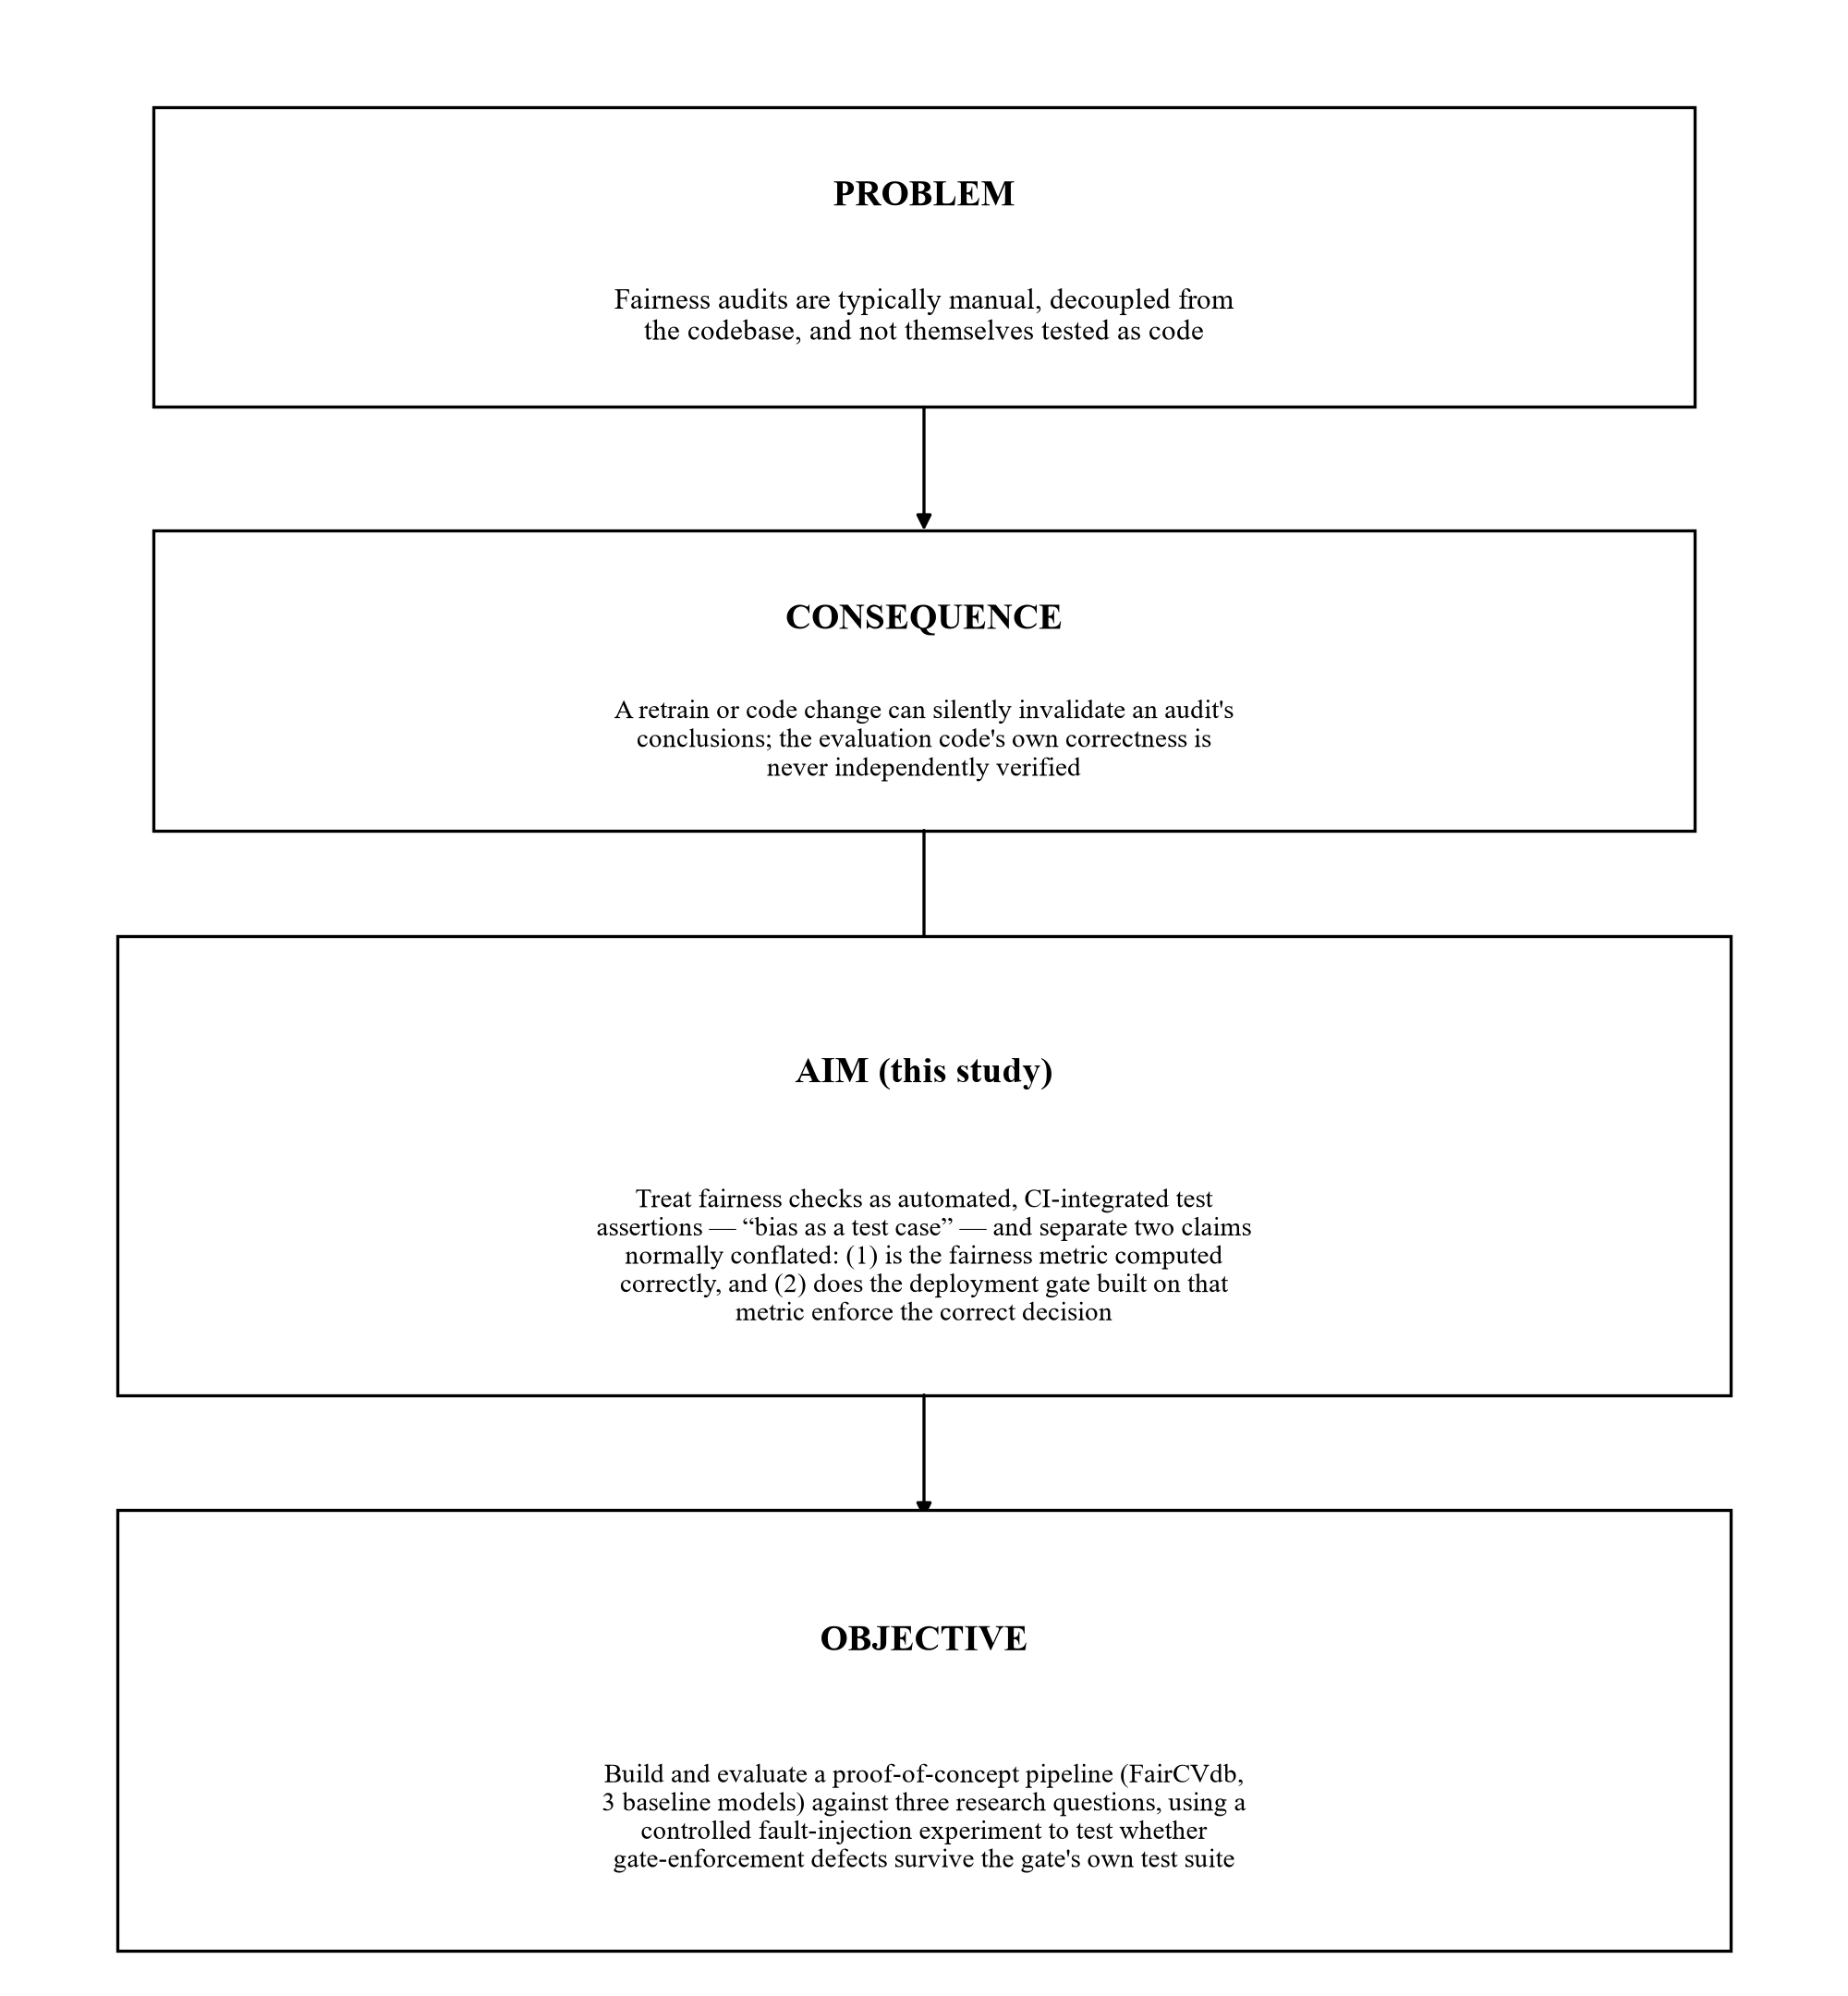
\includegraphics[width=\linewidth]{figures/fig1_problem_aim.png}
  \caption{The real-world problem motivating this study and its aim and objective.}\label{fig:problem}
\end{figure}

As summarized in \Cref{fig:problem}: manual, code-decoupled fairness audits can be silently invalidated by a retrain or code change; this study responds by treating fairness checks as CI-integrated test assertions and separating metric correctness from gate-enforcement correctness as independently testable claims.

\section{Related Work}\label{sec:RelatedWork}

\textbf{Fairness metrics.} Demographic parity and equalized odds are among the most widely used group fairness criteria \cite{Hardt2016,Dwork2012,Barocas2023}. Both are supported as first-class metrics in the fairlearn toolkit \cite{Bird2020} and in aequitas \cite{Saleiro2018}, the two libraries used in this work. It is well established that these criteria can conflict with one another and with predictive accuracy \cite{Kleinberg2017,Chouldechova2017}; this paper does not attempt to resolve that tension and instead treats threshold-based demographic parity and equalized odds checks as a representative, already-adopted pair of criteria to test the engineering pattern against. The broader space of group and individual fairness definitions, and the assumptions each encodes about what a model owes to whom, has itself been systematized as a taxonomy intended to help practitioners choose a criterion deliberately rather than by default \cite{Verma2018}; the present study takes that choice as given and instead asks a question upstream of it, whether the software enforcing whichever criterion is chosen does so correctly.

\textbf{FairCVdb.} Pe\~na et al. \cite{Pena2020} introduced FairCVdb as a synthetic benchmark for studying multimodal bias in automated r\'esum\'e screening, with paired blind, gender-biased, and ethnicity-biased scoring labels over the same 24,000 synthetic candidate profiles. Because the ground-truth bias mechanism is known by construction, FairCVdb is well suited to validating that a detection method correctly identifies bias whose presence or absence is already established, which is the role it plays here.

\textbf{Fairness testing as software testing.} Fairness testing of ML systems is by now a substantial research area in its own right; Chen, Zhang, Hort, Harman, and Sarro \cite{Chen2024} survey over 100 papers on the topic, organized by testing workflow and by what is being tested. Prior work has proposed treating fairness properties as testable software properties, including input-generation approaches for individual discrimination testing \cite{Galhotra2017,Udeshi2018} and mutation-based approaches that perturb data rather than code: Molinier, Temple, and Perrouin \cite{Molinier2024} introduce FairPipes, which applies mutation operators to sensitive attributes and their distributions, shuffling values or altering the distribution, to study how a model's fairness degrades as the data it sees after deployment drifts from its training distribution, evaluated across seven models and three datasets. These approaches, discrimination-input generation and data-distribution mutation alike, target the same layer as a fairness metric: does the model treat similar individuals differently, or does its fairness degrade under a changed input distribution. This paper is closely related in spirit but targets a different layer and a different mutation object: rather than mutating inputs or data to expose unfair model behavior, we inject faults into the software component that translates an already-computed fairness measurement into a deployment decision, and separately into the tests intended to verify that component. This gap is consistent with what practitioners themselves report: in an interview study of industry ML teams, Holstein, Vaughan, Daum\'e, Dud\'ik, and Wallach \cite{Holstein2019} find that practitioners lack tooling support for translating a computed fairness metric into a concrete engineering decision, and often improvise ad hoc checks rather than relying on a validated enforcement mechanism, which is precisely the gap between metric computation and gate enforcement this paper treats as a distinct testing target. To our knowledge this enforcement layer, whether the code that decides, on the basis of a fairness measurement, whether a model may be deployed is itself correct, is not the direct object of study in the fairness-testing literature surveyed above, which motivates treating it as a distinct testing target rather than assuming its correctness follows from the correctness of the underlying metric.

\textbf{Continuous integration and ML system testing.} The practice of running an automated test suite on every code change to catch regressions before they reach production is a long-standing software engineering discipline \cite{Fowler2006}. Its extension to machine learning systems specifically has been studied from an infrastructure and technical-debt perspective: Breck et al. \cite{Breck2017} frame ML testing as part of production readiness and propose a rubric of 28 tests and monitoring needs intended to reduce technical debt in production ML systems. This broader testing perspective motivates treating deployment-related checks as software-engineering concerns in their own right, rather than assuming that a successful model evaluation is sufficient; our work narrows that concern specifically to fairness enforcement, where the fairness result is computed separately and the software component that converts that result into a BLOCK or DEPLOY decision is tested as an independent artifact. Separately, recent work has operationalized AI assurance and governance requirements as executable, versioned policies with deterministic CI/CD gates: Muhammad, Yow, and Alsenan \cite{Muhammad2026} present Audit-as-Code, in which governance requirements, including fairness-related checks, are represented as executable policies that produce PASS, WARN, or BLOCK outcomes in a CI/CD pipeline. This confirms that executable fairness and assurance gates are already an established engineering direction; our focus is narrower still, treating the gate itself, once it exists, as a software component whose enforcement logic and covering test suite are subject to fault injection, rather than proposing or evaluating a new gating framework.

\textbf{Mutation testing.} Mutation testing evaluates a test suite's fault-detection capability by injecting small, syntactically valid faults (mutants) into the code under test and checking whether the existing tests fail in response; a mutant the suite fails to detect is said to have survived \cite{Jia2011}. We adopt this methodology, but apply it narrowly: rather than an exhaustive, tool-generated mutant set over the whole codebase, we hand-select seven mutants representative of the specific defect class motivating this paper (\Cref{sec:Results-RQ3}), which is a deliberate scoping choice discussed further in \Cref{sec:Limitations}.

\textbf{Positioning.} The distinction investigated here is deliberately narrower than fairness testing, mutation-based fairness testing, or executable fairness governance in general. Fairness testing, as surveyed above, is concerned with whether a model's predictions satisfy a fairness property; FairPipes is concerned with whether that property degrades under distributional drift; Audit-as-Code is concerned with representing assurance requirements as executable, versioned policy. This study instead treats the software component that translates an already-computed fairness result into a deployment decision as an explicit testing target in its own right, and evaluates whether representative faults in that component, and in the test suite intended to verify it, are detectable through the suite's own execution. To our knowledge, the work reviewed here does not directly evaluate the correctness of the software component that translates fairness measurements into deployment decisions, nor the fault-detection capability of the test suite intended to verify that component.

\section{Methodology}\label{sec:Method}

\begin{figure}[htbp]
  \centering
  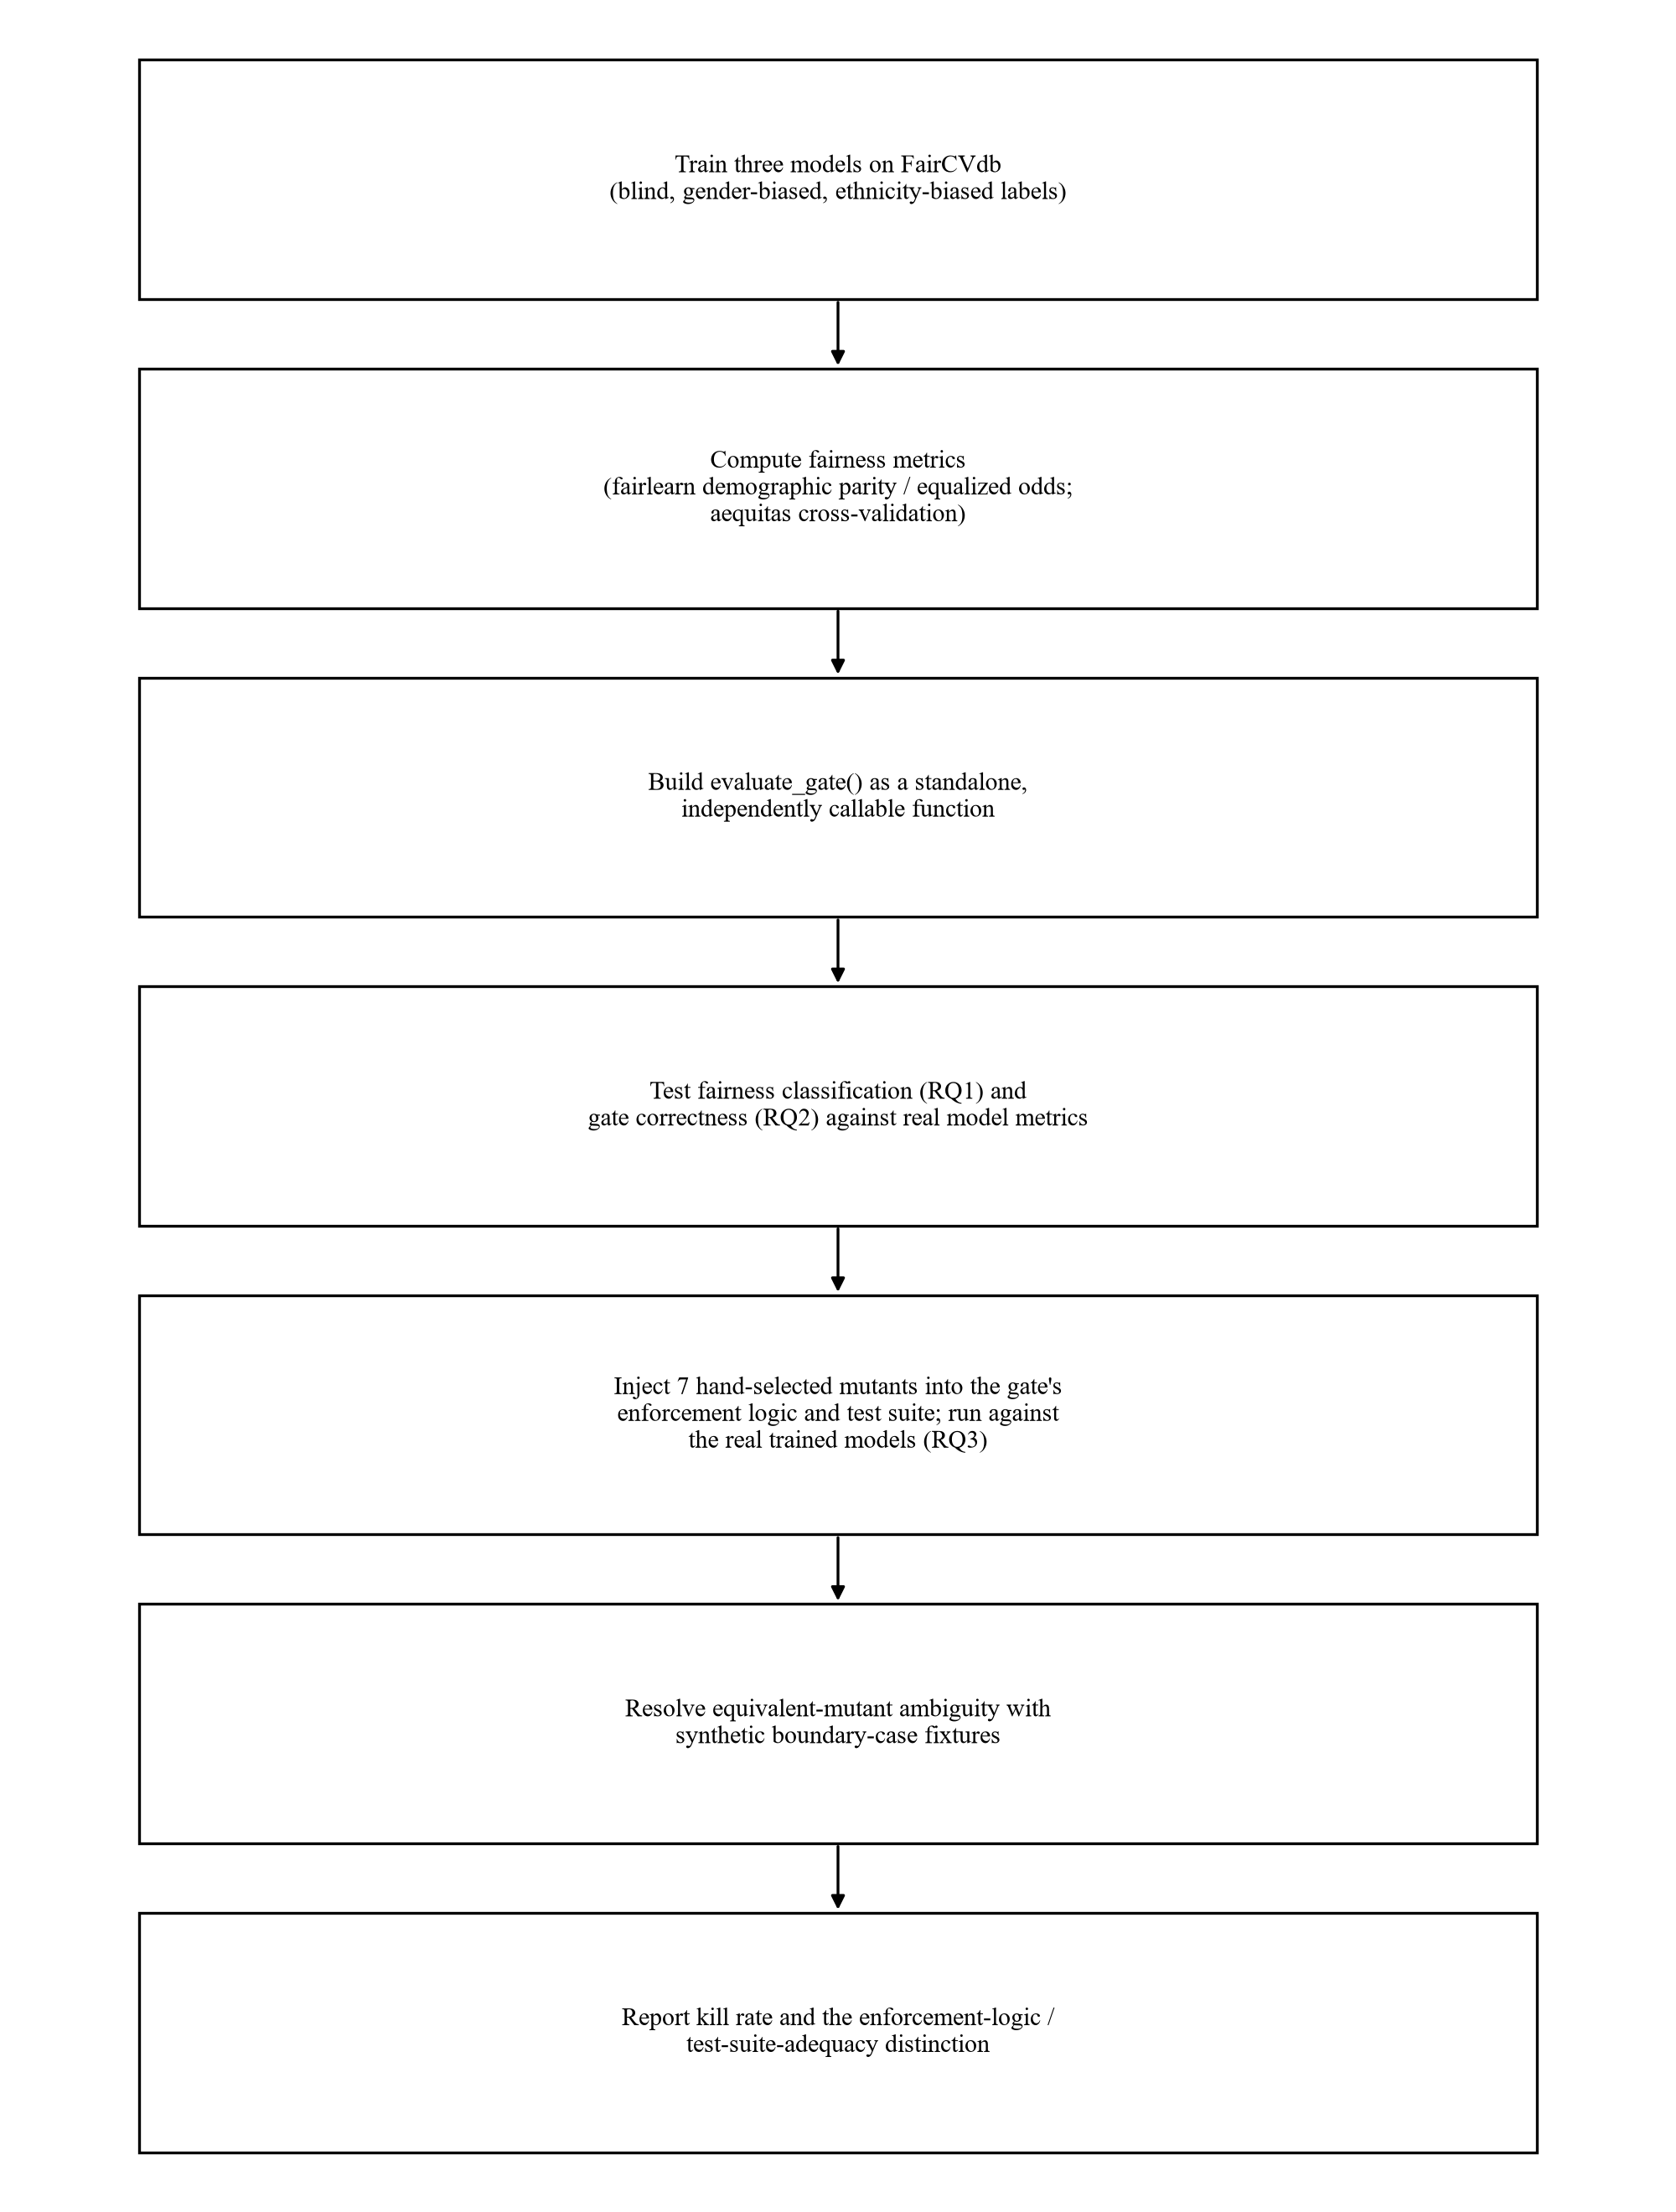
\includegraphics[width=\linewidth]{figures/fig2_approach.png}
  \caption{The study's approach, from model training through fault injection to the reported results.}\label{fig:approach}
\end{figure}

\Cref{fig:approach} summarizes the overall approach. \Cref{sec:Method-Dataset,sec:Method-Metrics,sec:Method-Pipeline,sec:Method-Validation} detail the dataset, metrics, and pipeline architecture; \Cref{sec:Results-RQ3} details the fault-injection procedure and the synthetic-fixture experiment that resolves equivalent-mutant ambiguity.

\subsection*{3.1 Dataset, labels, and models}\label{sec:Method-Dataset}

Baseline logistic regression classifiers were trained on FairCVdb \cite{Pena2020}, which provides 51-dimensional candidate profile features across 19,200 training and 4,800 test instances. Feature index 0 encodes ethnicity (three categories) and feature index 1 encodes gender (binary), directly, as columns of the profile vector supplied to the classifier; the dataset additionally provides gender/ethnicity-agnostic face-embedding features \cite{Pena2020} that this study does not use.

FairCVdb provides three parallel label sets over the same profiles: a blind target, constructed as a linear combination of competency and suitability attributes that deliberately excludes gender and ethnicity from the label-generation formula, and two biased targets (gender, ethnicity) constructed by applying a penalty factor to specific demographic groups on top of the blind target \cite{Pena2020}. It is important to state precisely what this means and does not mean for the present study: ``blind'' describes how the training label was generated, not which features the classifier receives. All three models evaluated here, including the blind-label model, are trained on the identical 51-dimensional profile vector, which includes the raw gender and ethnicity columns as input features. We therefore refer to the blind-label model throughout as the reference model rather than as ``the fair model'': it satisfies the fairness criteria evaluated in this study on this dataset at the stated threshold, because its label was not constructed using demographic penalties, but it is not blinded to demographic features at inference time, and no claim is made that it is fair in any broader or dataset-independent sense. This distinction is a direct response to a methodological ambiguity in an earlier draft of this work and is revisited as a limitation in \Cref{sec:Limitations}.

Three models were trained on this shared 51-dimensional feature set: a reference model on blind-target labels, a model on gender-biased-target labels, and a model on ethnicity-biased-target labels. Gender and ethnicity are used as the sensitive attribute in the corresponding fairness evaluation, drawn directly from feature indices 1 and 0 respectively.

\subsection*{3.2 Fairness metrics}\label{sec:Method-Metrics}

Two group fairness metrics were computed for each model:
\begin{itemize}
\item Demographic parity difference: the difference in positive prediction rate between the sensitive attribute's groups.
\item Equalized odds difference: the maximum difference in false positive rate or false negative rate between groups.
\end{itemize}

Both were computed using fairlearn 0.14.0 \cite{Bird2020}. A parallel cross-validation pass was performed using aequitas 1.1.0 \cite{Saleiro2018}, which independently computes disparity ratios (false positive rate disparity, false negative rate disparity, predicted positive rate disparity) relative to a reference group, providing a second, independently implemented measurement of the same underlying phenomenon.

A threshold of 0.10 was applied to both the demographic parity difference and the equalized odds difference to determine a binary pass/fail outcome. We treat this as an engineering policy parameter for the proof-of-concept gate, not a universally correct cutoff; disparity thresholds of this magnitude appear in the fairness literature \cite{Feldman2015}, but the two metrics are distinct quantities that need not share one defensible value in general.

\subsection*{3.3 Pipeline architecture}\label{sec:Method-Pipeline}

The enforcement decision is implemented as a standalone function, \texttt{evaluate\_gate(metrics)}, in \texttt{src/deployment\_gate.py}, independent of any test framework, shown in \Cref{listing:gate}:

\begin{code}
\caption{The gate's decision function, \texttt{evaluate\_gate()}}
\label{listing:gate}
\begin{minted}{python}
def evaluate_gate(metrics, dp_threshold=DP_THRESHOLD,
                   eo_threshold=EO_THRESHOLD):
    if (
        metrics["demographic_parity_difference"]
            >= dp_threshold
        or metrics["equalized_odds_difference"]
            >= eo_threshold
    ):
        return BLOCK
    return DEPLOY
\end{minted}
\end{code}

Equivalently, writing $dp$ and $eo$ for the measured demographic parity and equalized odds differences and $\tau_{dp} = \tau_{eo} = 0.10$ for the two thresholds, the gate decision is the predicate

\begin{quote}
$\mathrm{decision}(dp, eo) = \mathrm{BLOCK} \iff (dp \geq \tau_{dp}) \lor (eo \geq \tau_{eo})$, else $\mathrm{DEPLOY}$
\end{quote}

This form makes M2's fault explicit as a single symbolic substitution: replacing the disjunction $\lor$ with a conjunction $\land$ changes the predicate to $\mathrm{decision}(dp, eo) = \mathrm{BLOCK} \iff (dp \geq \tau_{dp}) \land (eo \geq \tau_{eo})$, which disagrees with the original on exactly the region where $dp$ and $eo$ fall on opposite sides of their thresholds, the region B2 and B3 are constructed to fall inside (\Cref{sec:Results-RQ3,fig:scatter}).

This is a deliberate architectural choice, not an incidental one. An earlier version of this pipeline inlined the equivalent condition directly inside a pytest assertion in the gate's test module (\Cref{sec:Method-Validation} describes a defect in that inline form). Extracting the decision into its own callable matters for the mutation-testing methodology in \Cref{sec:Results-RQ3}: it allows the gate's implementation to be mutated independently of the tests that check it, so that ``the gate's test suite catches a fault in the gate'' is a claim about two separate artifacts, not a test file checking a mutated copy of itself.

The evaluation is expressed as four pytest modules, corresponding to four distinct claims:

\textbf{Fairness-classification tests} (\texttt{test\_fairness.py}; 4 tests) assert that each model's fairness metrics fall on the expected side of the policy threshold given its known label construction: the gender-biased and ethnicity-biased models are asserted to fail the fairness threshold, and the reference model is asserted to pass it, for both sensitive attributes. We use ``fairness-classification'' rather than ``detection accuracy'' because these tests check fixed, known fixtures against a threshold rather than compute an accuracy statistic over a representative sample of models.

\textbf{Deployment gate tests} (\texttt{test\_deployment\_gate.py}; 3 tests) call \texttt{evaluate\_gate()} on the real, measured metrics for each model and assert the resulting decision: the gender-biased and ethnicity-biased models must be assigned BLOCK, and the reference model must be assigned DEPLOY. We simulate this logic rather than demonstrate it end-to-end: the GitHub Actions workflow described below runs the test suite on every push and uploads its results, but does not itself gate a separate deployment job, so no claim is made that this proof-of-concept is a working continuous deployment pipeline. It is a continuous integration pipeline whose test suite happens to check a deployment decision, and we use the term ``deployment gate'' only for the \texttt{evaluate\_gate()} function under test, not for the CI workflow itself.

\textbf{Gate boundary-case tests} (\texttt{test\_gate\_boundary\_cases.py}; 7 tests) call \texttt{evaluate\_gate()} directly on synthetic $(dp, eo)$ pairs rather than on metrics computed from a trained model: one metric breaching threshold while the other does not, both breaching, neither breaching, and the exact-threshold edge on each metric (the gate's comparison is $\geq$, so a value equal to the threshold must still BLOCK). These exist because the three real trained models happen to breach both fairness metrics whenever they breach either one, so the model-based deployment-gate tests alone cannot distinguish a gate that requires either metric to breach threshold from one that requires both to, precisely the ambiguity \Cref{sec:Results-RQ3} resolves for mutant M2 with a synthetic-fixture experiment inside the mutation harness. This module puts the same synthetic cases into the committed test suite itself, as permanent regression coverage rather than only a mutation-testing side experiment.

A fourth module (\texttt{test\_aequitas\_crossvalidation.py}; 2 tests) repeats the gender-bias detection check using the independently implemented aequitas metrics as a cross-check on the fairlearn-based result. In total the suite comprises 16 tests across the four modules.

The separation between the first two modules is deliberate. A fairness-classification test can pass while a deployment-gate test built on the same underlying metric computation fails, or vice versa, if \texttt{evaluate\_gate()} does not correctly consume the metric's output. Conflating the two into a single test class would leave this class of defect undetected. All four modules are executed on every push and pull request via a GitHub Actions workflow, with results persisted as a JSON artifact for traceability across runs; as noted above, this workflow is a continuous integration check, not a deployment pipeline.

\subsection*{3.4 Implementation validation}\label{sec:Method-Validation}

During development, a directional defect was identified in the deployment gate test for the gender-biased model, at the time the decision logic was still inlined directly inside the test rather than factored into \texttt{evaluate\_gate()}. The original gate test contained two separate assertions, one for each metric, both pointing the same wrong direction, reproduced in \Cref{listing:defect}:

\begin{code}
\caption{The original, defective inline assertions}
\label{listing:defect}
\begin{minted}{python}
assert metrics["demographic_parity_difference"] \
    < DP_THRESHOLD, \
    f"BLOCKED: demographic parity violation " \
    f"({metrics['demographic_parity_difference']:.3f})"
assert metrics["equalized_odds_difference"] \
    < EO_THRESHOLD, \
    f"BLOCKED: equalized odds violation " \
    f"({metrics['equalized_odds_difference']:.3f})"
\end{minted}
\end{code}

Each assertion evaluated whether its respective metric was below threshold, which is the condition for the model to be treated as deployable, when the intended behavior, consistent with the test's own docstring (``biased gender model should FAIL this gate''), was for the biased model to be rejected. Executing the test suite surfaced the defect directly: the gate correctly measured a demographic parity difference of 0.146 on the biased model, exceeding the 0.10 threshold as intended, the inverted assertion caused pytest to report the test as failed even though the measured disparity correctly exceeded the policy threshold. The metric computation itself was not at fault: $0.146 < 0.10$ evaluates correctly to false. What was wrong was the direction of the condition each assertion attached to its comparison. The fix replaced the two independent \texttt{<}-threshold assertions with a single condition requiring that at least one of the two disparity metrics meet or exceed threshold for the model to be treated as correctly blocked, later factored out into the standalone \texttt{evaluate\_gate()} function shown in \Cref{sec:Method-Pipeline}.

An equivalent gate test was added for the ethnicity-biased model, which had no prior gate coverage.

This single observed defect motivates, but does not by itself establish, the paper's central claim (RQ3). \Cref{sec:Results-RQ3} reports a controlled fault-injection experiment designed to test that claim more systematically.

\section{Results}\label{sec:Results}

\subsection*{4.1 RQ1: Fairness classification}\label{sec:Results-RQ1}

\Cref{tab:fairness} reports demographic parity difference and equalized odds difference for each of the three baseline models, measured against the FairCVdb test split ($n = 4{,}800$), using the corresponding sensitive attribute for each biased model.

\begin{table}[ht]
    \caption{Fairness metrics by model and protected attribute (threshold = 0.10 for both metrics).}
    \label{tab:fairness}
    \centering
    \footnotesize
    $\begin{tabu}{llll}
        \toprule
        \text{Model} & \text{Protected attribute} & \text{Demographic parity }\Delta & \text{Equalized odds }\Delta \\
        \midrule
        \text{Gender-biased} & \text{gender} & 0.146 & 0.607 \\
        \text{Ethnicity-biased} & \text{ethnicity} & 0.450 & 0.659 \\
        \text{Reference (blind-label)} & \text{gender / ethnicity} & 0.020 & 0.033 \\
        \bottomrule
    \end{tabu}$
\end{table}

Both biased models exceed the 0.10 threshold on both metrics, while the reference model remains below it on both, consistent with the intended distinction between the biased and blind label constructions (\Cref{sec:Method-Dataset}). These are measured outcomes of the trained classifiers, not a result guaranteed by label construction alone; a model could in principle be trained on a biased-target label and still fail to reproduce that bias's effect on its predictions, or vice versa. The margin is substantially larger for the ethnicity-biased model (0.450) than the gender-biased model (0.146) on demographic parity, suggesting the induced bias is not uniform in magnitude across the two protected attributes in this dataset, though we did not investigate the source of this asymmetry further and note it as a direction for future work rather than a finding in itself.

The aequitas cross-validation pass independently computed an elevated false negative rate disparity for the female group under the gender-biased model, providing an independent implementation-level cross-check of the disparity measurement rather than an independent proof that the reference model is fair in any absolute sense.

All 4 fairness-classification tests and both aequitas cross-validation tests pass, indicating that the fairness-classification layer produces the expected outcomes for the biased and reference models on these fixtures (RQ1: affirmative, within the scope of \Cref{sec:Limitations}'s limitations).

\subsection*{4.2 RQ2: Deployment-gate correctness}\label{sec:Results-RQ2}

Following the correction described in \Cref{sec:Method-Validation}, all 3 deployment-gate tests pass: both biased models are correctly rejected, and the reference model is correctly accepted (RQ2: affirmative, post-correction). This result alone does not establish that the gate generally enforces fairness-test outcomes correctly, only that it does so on the three fixtures currently under test. The 7 gate boundary-case tests (\Cref{sec:Method-Pipeline}) extend this beyond the real models' specific metric values: all pass, including the exact-threshold edge and the case where only one of the two metrics breaches threshold, which the three model-based fixtures alone do not exercise (\Cref{sec:Results-RQ3} returns to why this particular gap matters). \Cref{sec:Results-RQ3} probes gate correctness more adversarially still, via fault injection rather than direct assertion.

\subsection*{4.3 RQ3: Fault injection into the gate}\label{sec:Results-RQ3}

To evaluate RQ3 systematically rather than relying on the single defect reported in \Cref{sec:Method-Validation}, seven mutants were injected and each executed against the real trained models and the real FairCVdb test split. Because \texttt{evaluate\_gate()} is now a standalone function (\Cref{sec:Method-Pipeline}), the two fault layers are injected into two different artifacts rather than both into the test file. Enforcement-logic mutants (M1, M2, M5, M7) patch a copy of \texttt{src/deployment\_gate.py} itself, changing the decision computed from a given, correctly measured metric value (a comparison operator, a threshold, a Boolean combinator, the BLOCK/DEPLOY return values), and the real, unmodified \texttt{test\_deployment\_gate.py} suite is run against the patched module. Test-suite-adequacy mutants (M3, M4, M6) patch a copy of \texttt{test\_deployment\_gate.py} instead, leaving \texttt{evaluate\_gate()} untouched, since these faults are about whether the suite adequately exercises a correct gate (a dropped test case, an assertion that cannot fail, a test fixture that reads the wrong feature column), not about a fault in the gate's own decision logic. A mutant is caught if the resulting test run no longer reports results consistent with the known ground truth (both biased models BLOCKed, reference model DEPLOYed); a mutant survives if it still does despite the injected fault. This is a hand-selected fault set representative of the defect class in \Cref{sec:Method-Validation}, not an exhaustive or tool-generated mutation sweep (see \Cref{sec:Limitations}).

\begin{algorithm}[htbp]
\caption{Fault-injection procedure, applied once per mutant $M_i$}
\label{alg:faultinjection}
\begin{algorithmic}[1]
\Require mutant $M_i$ with target artifact $A_i \in \{\text{gate}, \text{test}\}$; real trained models; ground truth $G$ (biased $\rightarrow$ BLOCK, reference $\rightarrow$ DEPLOY)
\Ensure verdict $\in \{\text{caught}, \text{survived}\}$
\If{$A_i = \text{gate}$}
    \State $G' \gets \Call{patch}{\text{deployment\_gate.py}, M_i}$ \Comment{enforcement-logic mutant}
    \State $run \gets \Call{pytest}{\text{test\_deployment\_gate.py}, \text{gate}=G'}$ \Comment{real, unmodified tests}
\Else
    \State $T' \gets \Call{patch}{\text{test\_deployment\_gate.py}, M_i}$ \Comment{test-suite-adequacy mutant}
    \State $run \gets \Call{pytest}{T', \text{gate}=\text{deployment\_gate.py}}$ \Comment{real, unmodified gate}
\EndIf
\If{$run.result \neq G$}
    \State \Return caught \Comment{mismatch: pytest reports a failure}
\Else
    \State \Return survived \Comment{run still matches ground truth despite $M_i$}
\EndIf
\end{algorithmic}
\end{algorithm}

\begin{figure}[htbp]
  \centering
  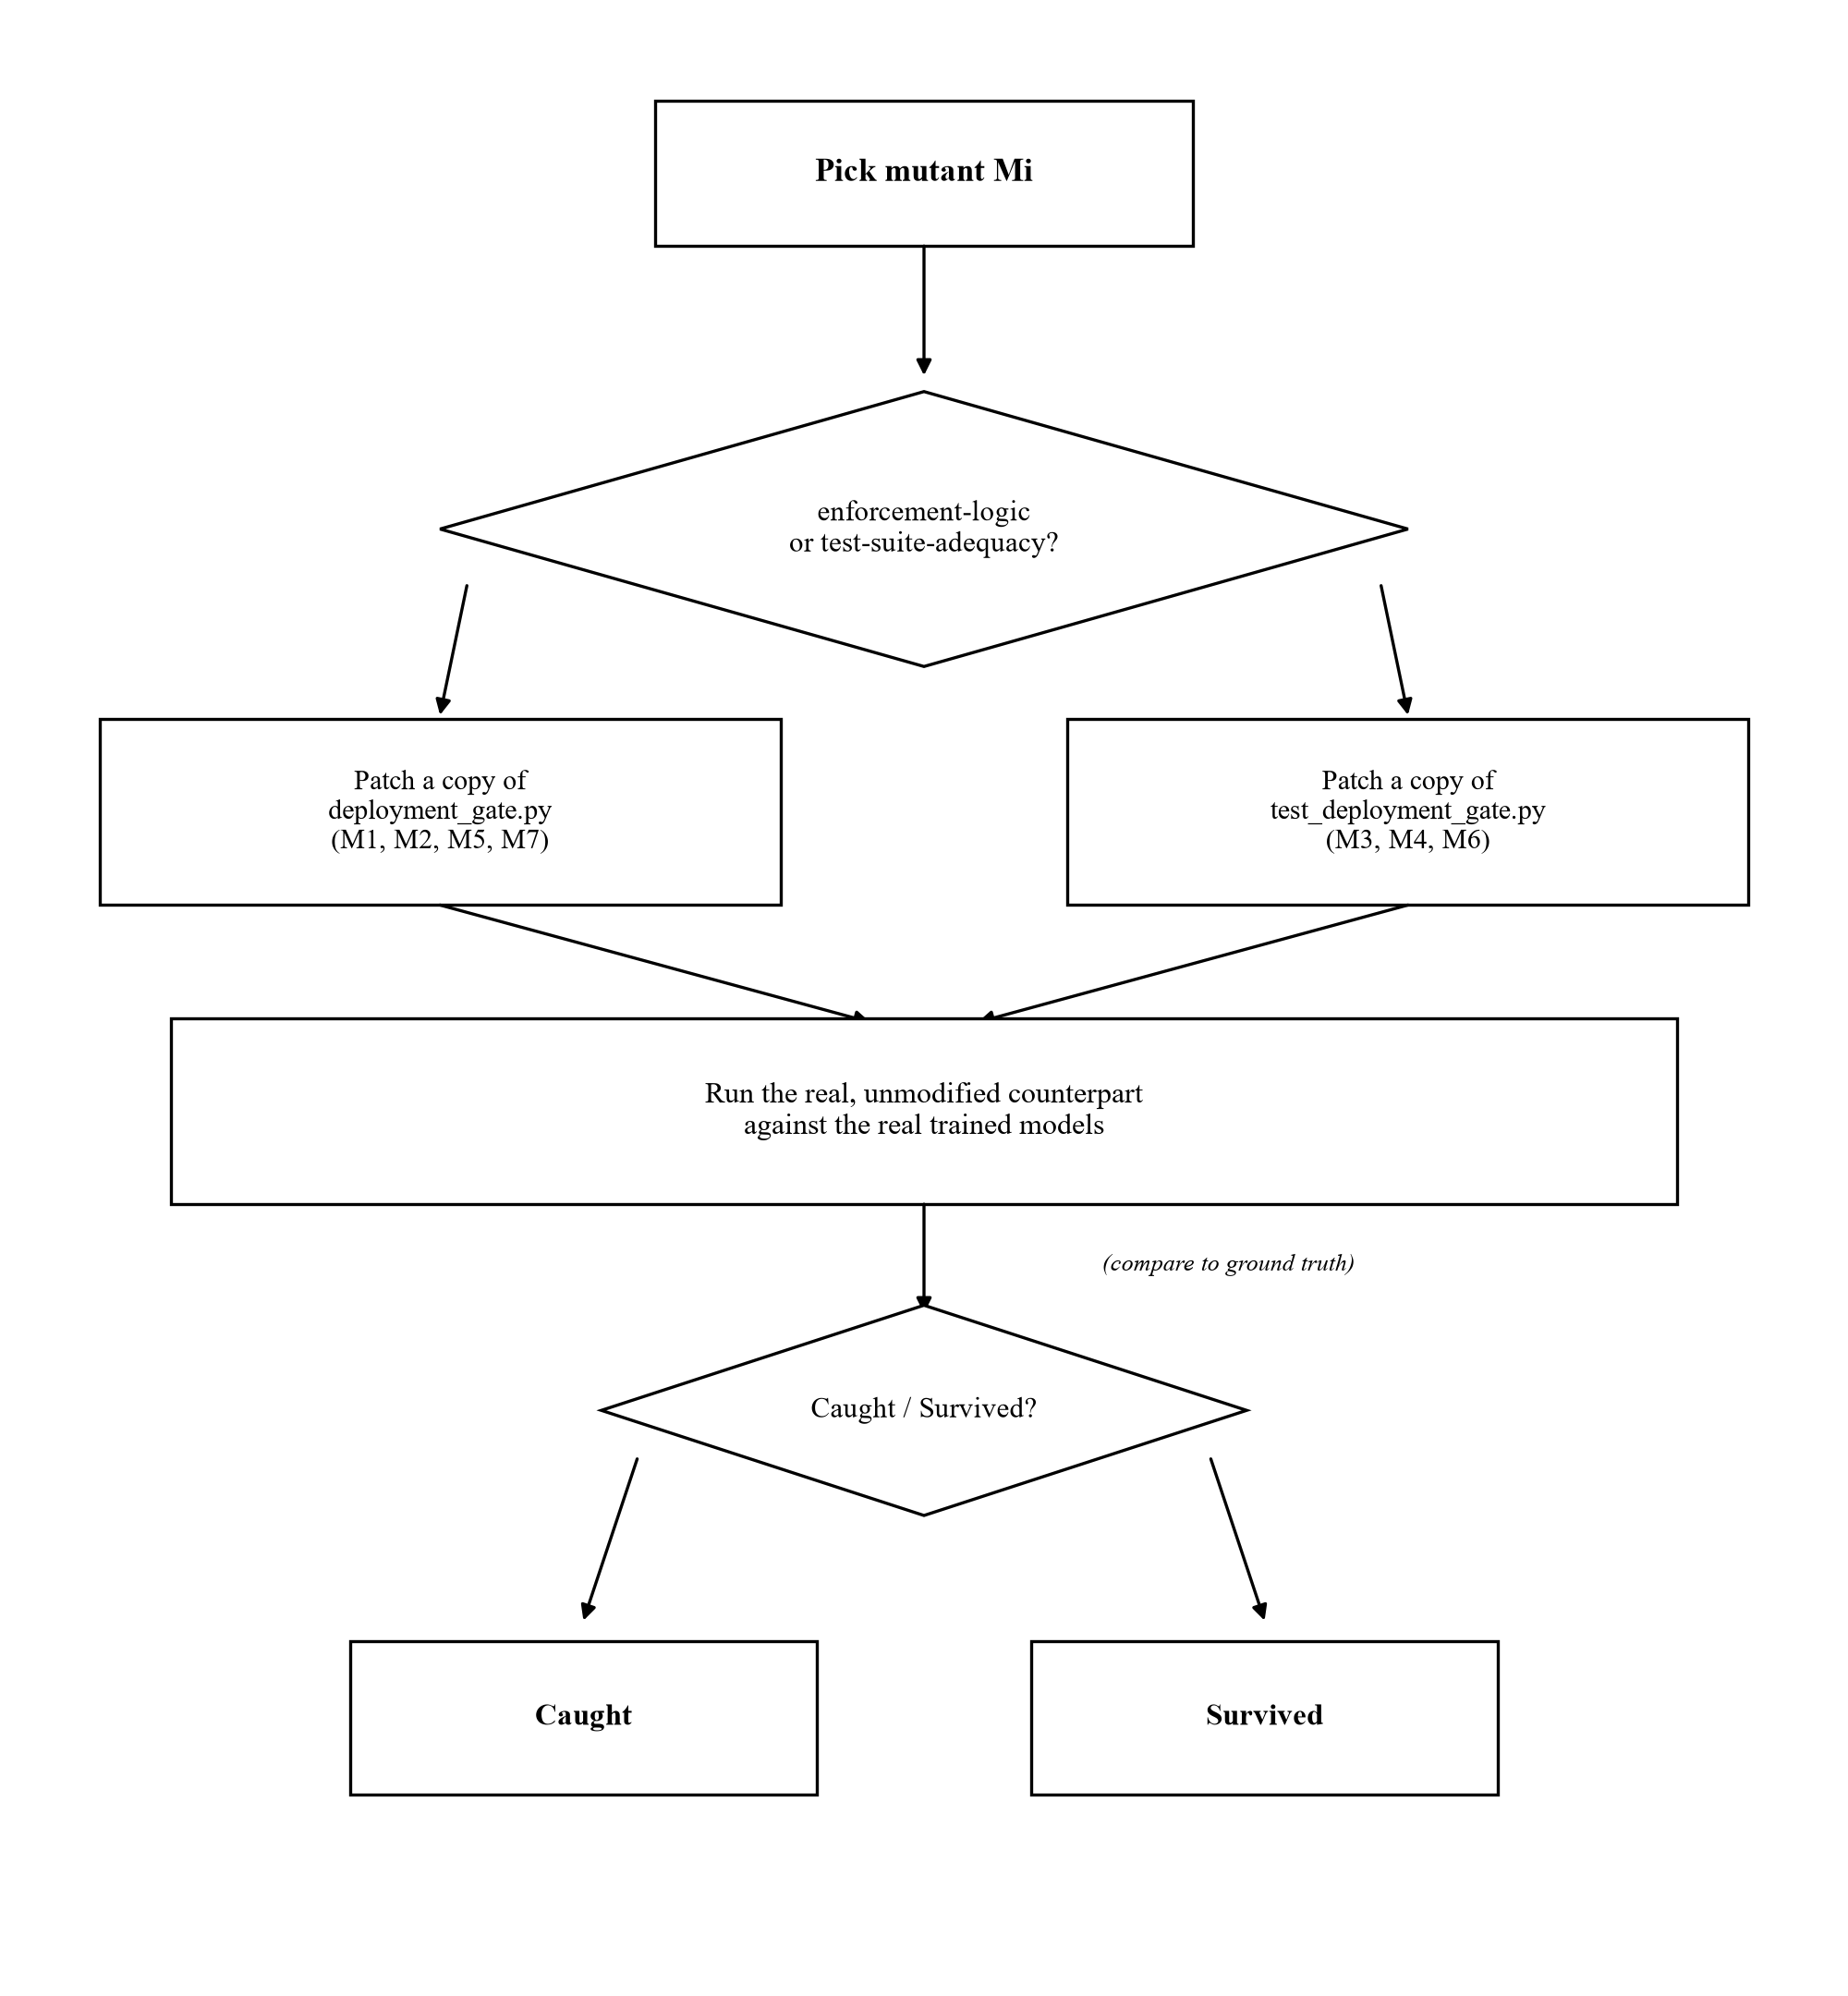
\includegraphics[width=\linewidth]{figures/fig3_faultinjection.png}
  \caption{The fault-injection procedure applied to each of the seven mutants.}\label{fig:faultinjection}
\end{figure}

\Cref{fig:faultinjection} illustrates the procedure of \Cref{alg:faultinjection}, applied once per mutant (M1--M7); the split at the top determines which artifact is patched and which real, unmodified counterpart is run against it. Full results in \Cref{tab:mutants}.

\begin{table}[ht]
    \caption{Fault-injection results (7 mutants, real models, real data). Kill rate: 4/7 (57\%); by fault layer, 3/4 enforcement-logic mutants caught, 1/3 test-suite-adequacy mutants caught. *M2's survival is resolved by Experiment 2 (\Cref{tab:synthetic,fig:scatter}) below.}
    \label{tab:mutants}
    \centering
    \footnotesize
    \begin{tabularx}{\columnwidth}{@{}llX l@{}}
        \toprule
        Mutant & Layer & Injected fault & Result \\
        \midrule
        M1 & enforcement & Flip $\geq$ to $<$ (retains OR combinator) & Caught \\
        M2 & enforcement & Change OR to AND combinator & Survived* \\
        M3 & test-suite & Delete the ethnicity gate test entirely & Survived \\
        M4 & test-suite & Swap sensitive-attribute column (idx 1 not 0) & Caught \\
        M5 & enforcement & Widen both thresholds from 0.10 to 0.90 & Caught \\
        M6 & test-suite & Replace gender assertion with \texttt{assert True} & Survived \\
        M7 & enforcement & Swap the BLOCK/DEPLOY return values & Caught \\
        \bottomrule
    \end{tabularx}

    \smallskip
    \footnotesize enforcement = enforcement-logic mutant (patches \texttt{deployment\_gate.py}); test-suite = test-suite-adequacy mutant (patches \texttt{test\_deployment\_gate.py}).
\end{table}

\begin{figure}[htbp]
  \centering
  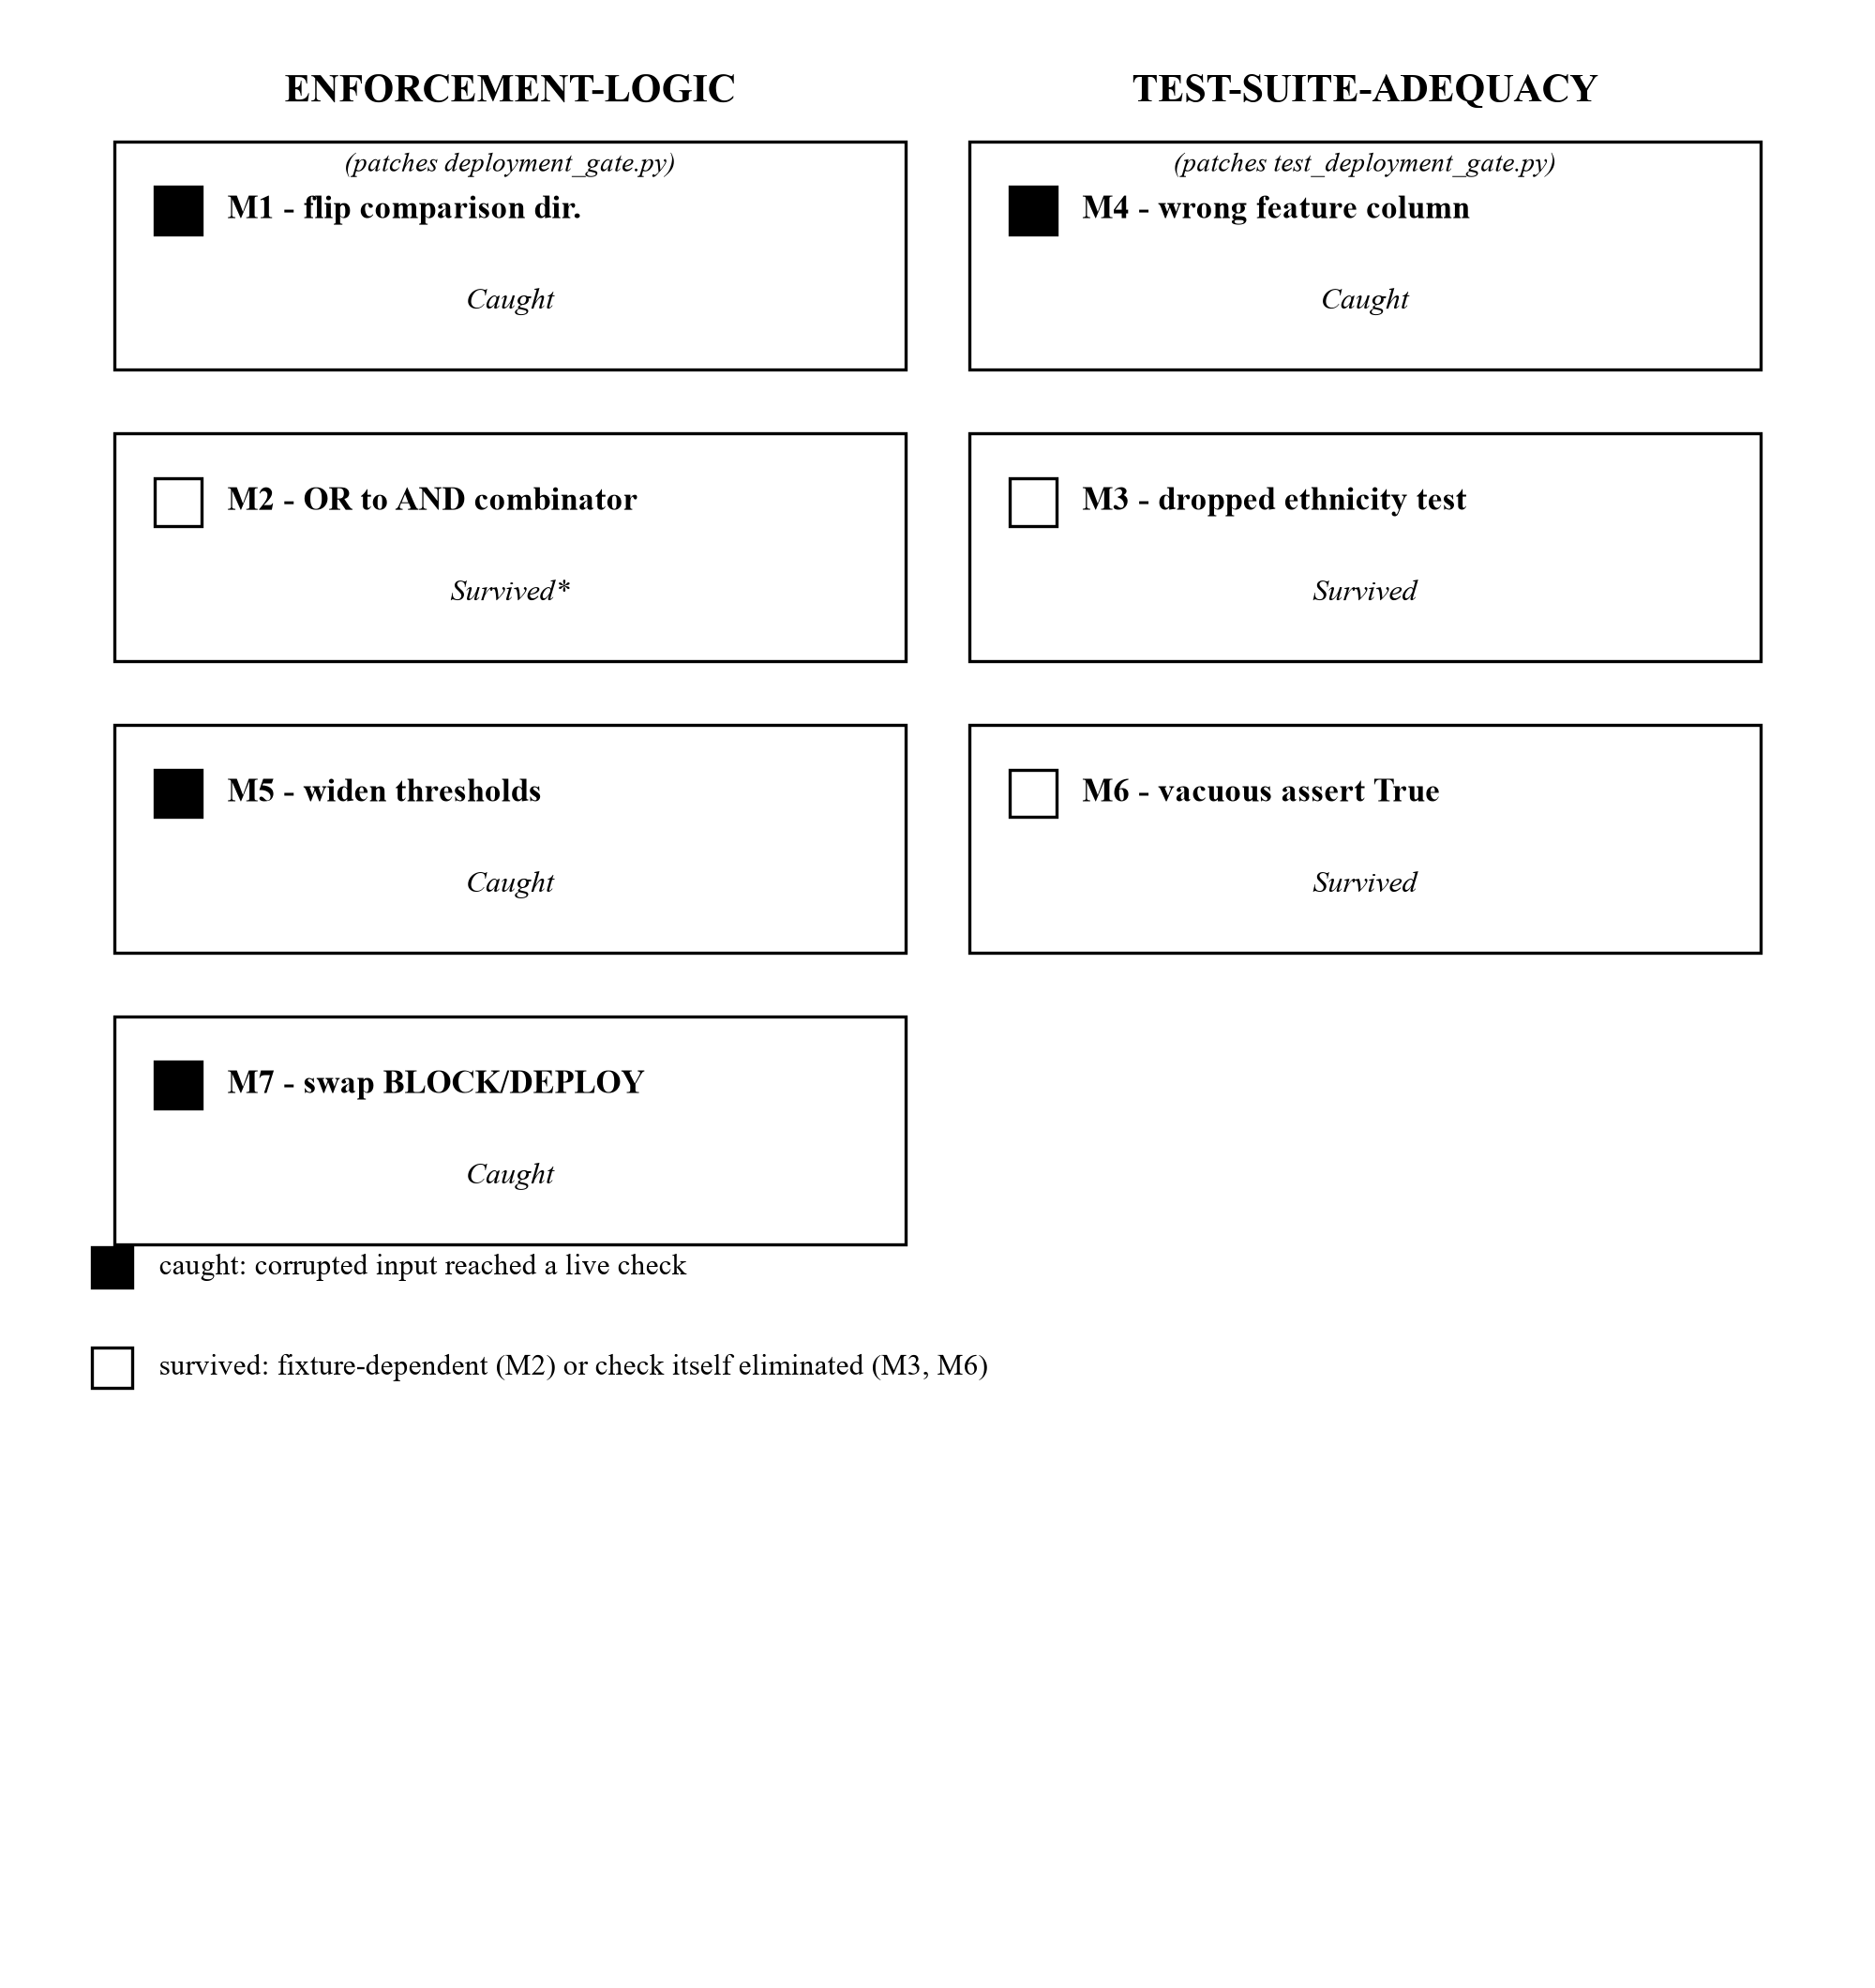
\includegraphics[width=\linewidth]{figures/fig4_mutantgrid.png}
  \caption{The seven mutants sorted by fault layer and outcome.}\label{fig:mutantgrid}
\end{figure}

As \Cref{fig:mutantgrid} shows, M4 sits in the test-suite-adequacy column but is caught, because it corrupts a test's input rather than removing the check; M2 sits in the enforcement-logic column but survives here, resolved separately in \Cref{tab:synthetic} and \Cref{fig:scatter}. Layer and outcome are independent axes, not the same distinction.

Four of the seven mutants were caught. M4 is worth noting separately from the other enforcement-logic mutants: although it is classified as a test-suite-adequacy fault (it patches the test file, not the gate module, and the gate's own decision logic is never at fault here), it is caught, because reading the wrong feature column produces a metric value that the correct, unmutated \texttt{evaluate\_gate()} correctly rejects on. This illustrates that ``test-suite-adequacy'' and ``detectable by the suite'' are not the same axis: a fault in a test's fixture can still be caught if it happens to produce an assertion failure, whereas M3 and M6 cannot be caught through the suite's own pass/fail signal by any fixture, because they remove the assertion itself rather than corrupting its input. M2, an enforcement-logic fault, survives for a third and different reason worth separating out.

M2 changes the gender gate's Boolean combinator from OR to AND: the mutated gate rejects a model only if both metrics breach threshold, rather than either one. On the real models used in this study, M2 survives, both real biased-model fixtures happen to breach both demographic parity and equalized odds simultaneously, so OR and AND agree on every fixture the existing suite exercises. This raises a standard concern in mutation testing: a surviving mutant may be a genuine gap, or it may be an equivalent mutant whose behavior is indistinguishable from the original on the available test data \cite{Jia2011}. To resolve which is the case here, we ran a second, synthetic-fixture experiment: four hand-picked (demographic parity, equalized odds) pairs, constructed independently of any trained model, chosen so that two of them (B2, B3) breach exactly one metric and not the other.

\begin{table}[ht]
    \caption{Synthetic (dp, eo) fixtures distinguishing the OR and AND gate combinators (threshold = 0.10).}
    \label{tab:synthetic}
    \centering
    \footnotesize
    $\begin{tabu}{llllll}
        \toprule
        \text{Fixture} & dp & eo & \text{Orig. (OR) rejects?} & \text{M2 (AND) rejects?} & \text{Distinguishes M2?} \\
        \midrule
        \text{B1 (both breach)} & 0.146 & 0.607 & \text{Yes} & \text{Yes} & \text{No} \\
        \text{B2 (DP only)} & 0.146 & 0.050 & \text{Yes} & \text{No} & \text{Yes} \\
        \text{B3 (EO only)} & 0.050 & 0.607 & \text{Yes} & \text{No} & \text{Yes} \\
        \text{B4 (neither breach)} & 0.020 & 0.030 & \text{No} & \text{No} & \text{No} \\
        \bottomrule
    \end{tabu}$
\end{table}

\begin{figure}[htbp]
  \centering
  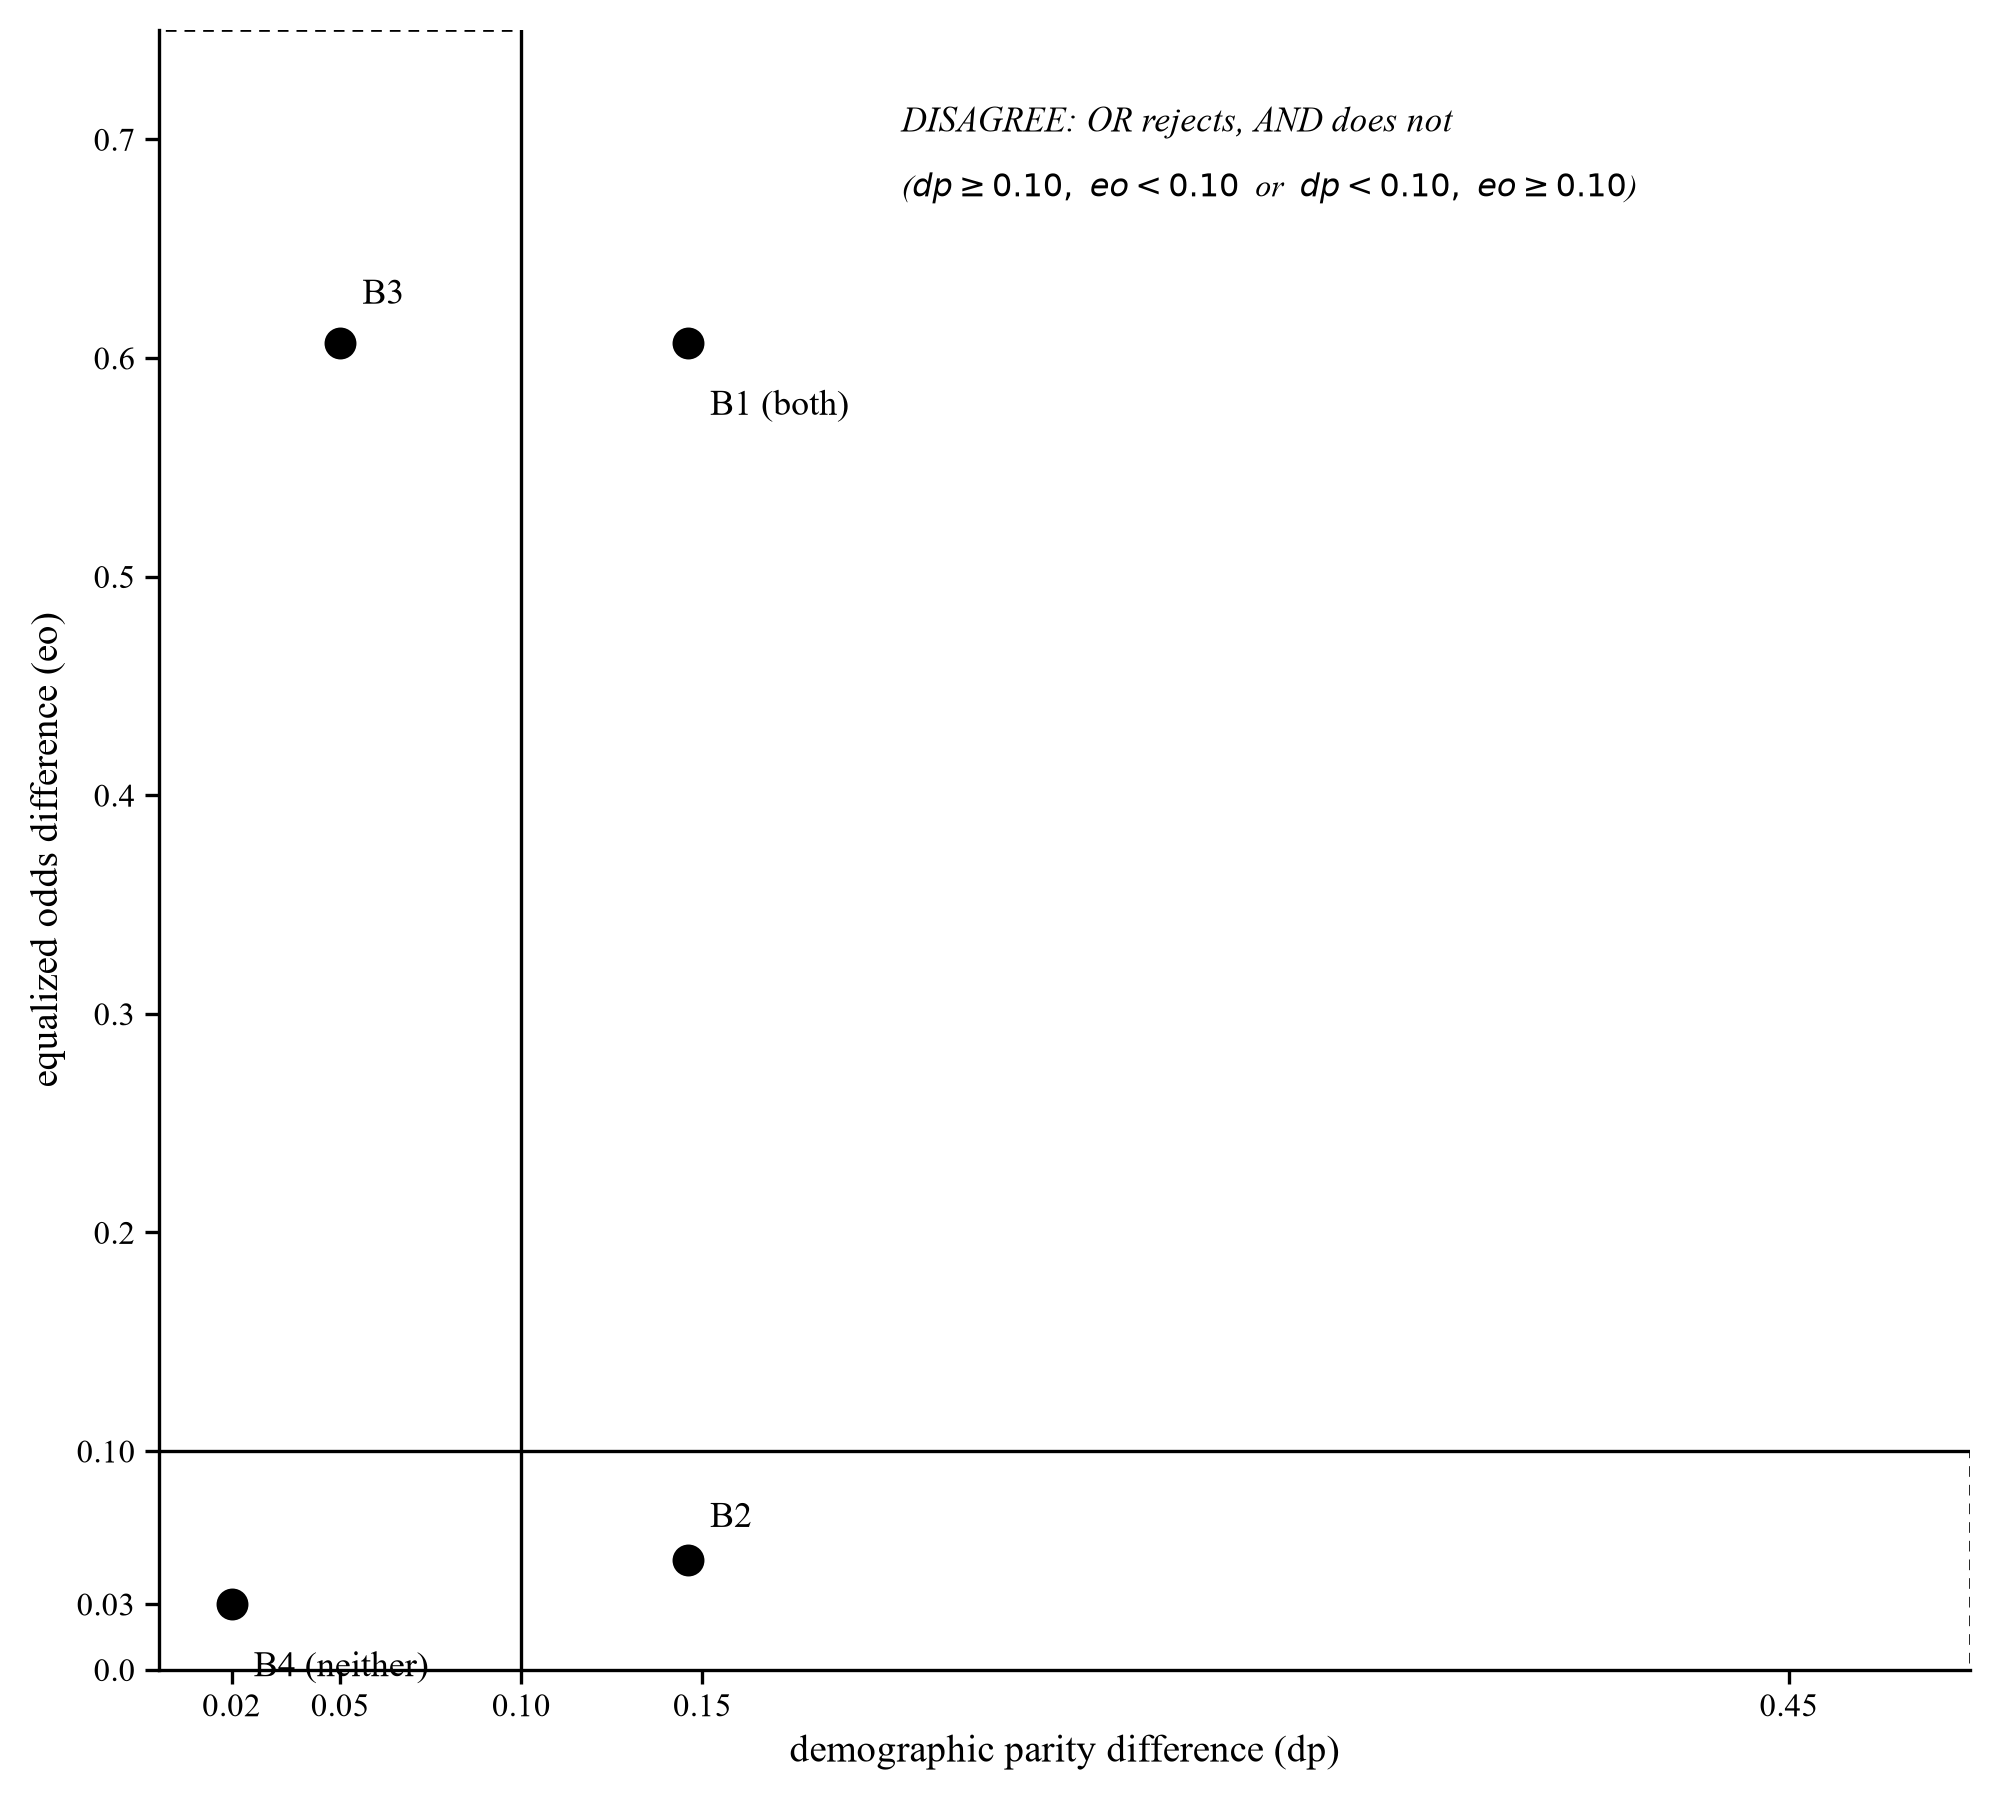
\includegraphics[width=\linewidth]{figures/fig5_scatter.png}
  \caption{Where the OR and AND gate combinators disagree, plotted against the B1--B4 fixtures.}\label{fig:scatter}
\end{figure}

In \Cref{fig:scatter}, darker shading marks the two quadrants where OR rejects but AND does not, exactly one metric over threshold. B2 and B3 fall inside them and distinguish M2; B1 (both metrics over) and B4 (neither) fall in quadrants where OR and AND agree, which is why the three real trained models, which all land in the corner-agreeing region, never exercised the disagreement.

B2 and B3 confirm that OR and AND are not, in general, equivalent: whenever exactly one metric breaches threshold, the two combinators produce opposite deploy/reject decisions. M2's survival in Experiment 1 is therefore an artifact of this particular dataset's real models both breaching both metrics together, not a property of the gate logic itself. This distinction matters for how the result should be read: M2 is a real semantic difference that the current fixture set happens not to exercise, which is a data-coverage limitation of the fixtures rather than a logic error in the gate as evaluated, whereas M3 and M6 cannot be resolved by adding more fixtures of the same kind, since no fixture value can make a deleted test run or a vacuous assertion fail.

So RQ3's answer is not simply ``enforcement-logic faults are detectable, test-suite-adequacy faults are not'': M4 breaks that pattern by being caught anyway. What holds instead is narrower and, we think, more useful: whether a fault corrupts an input to a check that still executes, or eliminates the check outright. Only the latter is structurally undetectable through the suite's own signal, and catching it needs something external: coverage-directed code review, a required-coverage policy in CI, or the fault-injection procedure used here.

\section{Discussion}\label{sec:Discussion}

\Cref{fig:pipeline} puts the two halves of \Cref{sec:Method,sec:Results} side by side: the pipeline a fairness decision actually flows through, and the tests that check each part of it from the outside, not as further steps the decision passes through, but as independent validators sitting alongside it.

\begin{figure}[htbp]
  \centering
  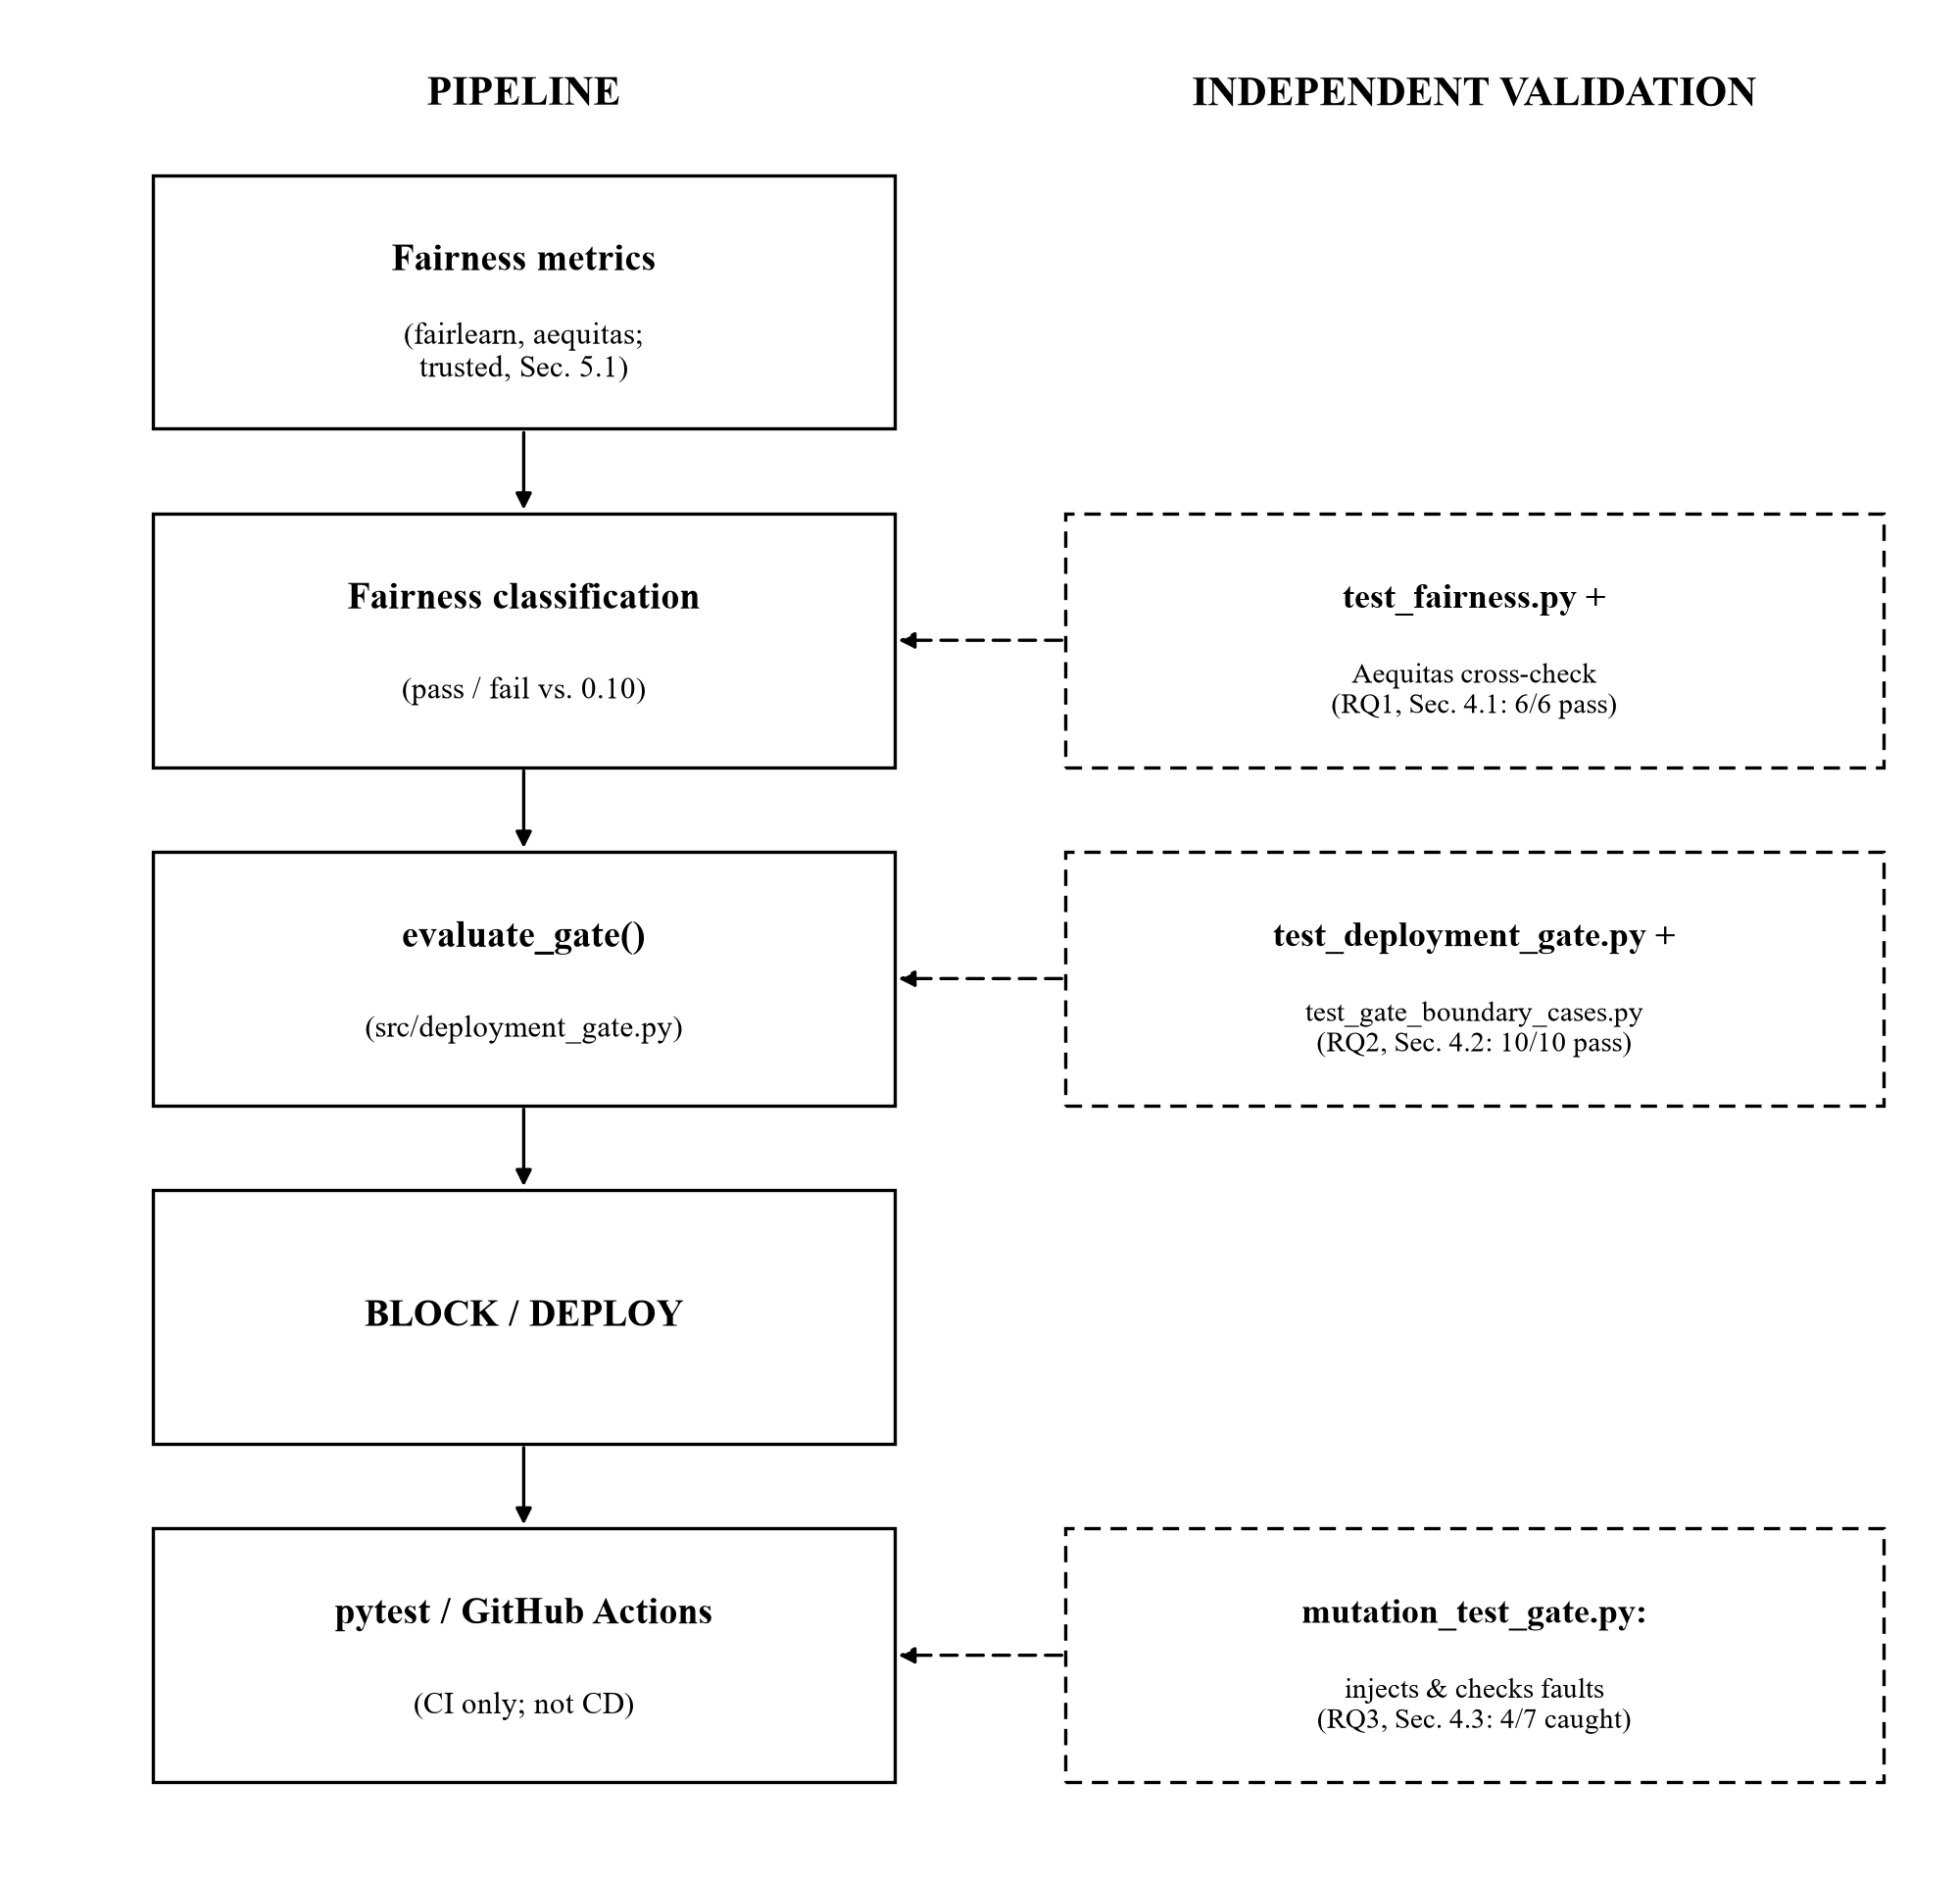
\includegraphics[width=\linewidth]{figures/fig6_pipeline.png}
  \caption{The fairness-decision pipeline (left) and the tests that independently validate each part of it (right).}\label{fig:pipeline}
\end{figure}

The right column are checks on the left column, not further pipeline stages (dashed borders mark the independent-validation boxes). A defect in \texttt{evaluate\_gate()} can pass fairness classification; a passing gate test can still miss faults the mutation experiment exposes; and the mutation experiment itself is scoped to a hand-selected fault set (\Cref{sec:Limitations}). CI enforcement of the gate's result against a real deployment step is not evaluated.

The point of this paper is not that demographic parity or equalized odds are hard to compute; \Cref{tab:fairness}'s margins are wide enough that any reasonable threshold catches them, and both libraries are treated as trusted instruments rather than independently re-derived (\Cref{sec:Limitations}). The point is that the code acting on a correct fairness outcome is itself a place things can go wrong, independent of the outcome's correctness, and that this only becomes visible once the gate is tested as its own claim. Within that, the M4 versus M3/M6 split from \Cref{sec:Results-RQ3} is the sharper lesson: what determines whether a fault is caught is not which side of the gate/test boundary it sits on, but whether it corrupts a value flowing into a live check or erases the check itself.

Practically, this means a fairness score being computed and logged is not enough; the code consuming it to make a deploy decision needs its own tests against the same fixtures, and needs to exist as something callable and mutable on its own (\Cref{sec:Method-Pipeline}), not logic buried inside the assertion checking it. The gate itself, once built, is a legitimate testing target with its own failure modes. An implementation that only logs a score would let a defect like \Cref{sec:Method-Validation}'s, or an M2/M3/M6-style fault, pass silently, a correct-looking number next to a gate that no longer does anything. And because check-eliminating faults are invisible to the suite's own signal by construction, catching them takes something outside the suite: coverage auditing, a required-coverage CI policy, or fault-injection like the kind used here.

\section{Conclusions}\label{sec:Conclusions}

This paper investigated two claims a fairness-testing pipeline must validate independently: the fairness-classification layer produces the expected classification on the tested fixtures using the metric implementations, and the deployment gate correctly translates those outcomes into the expected deploy/reject decisions. To make that distinction more than a conceptual one, the gate's decision logic was pulled out into a standalone function, \texttt{evaluate\_gate()}, rather than left inlined inside the assertion that checks it.

On FairCVdb, both claims held within the scope of the tested fixtures: the fairness-classification layer produced the expected outcomes for the biased and reference models, and the gate, once the directional defect found during development was corrected, correctly translated those outcomes into deploy/reject decisions. The more interesting result came from testing the gate adversarially, via fault injection, rather than trusting that it passed. Four of seven mutants were caught. The three that weren't split into two different kinds of gap: one gate-logic mutant (OR to AND) survived only because this dataset's real biased models happen to breach both fairness metrics at once, a synthetic fixture killed it once we deliberately built a case where only one metric breached; the other two, a dropped test and a disabled assertion, could not have been caught by any fixture, because there was no longer a check for any input to trigger.

The general lesson is narrower than ``test everything twice'': in the faults examined here, detectability through the suite's own pass/fail signal depended on whether a fault corrupted a value reaching a check that still ran or removed the check itself, regardless of which side of the gate/test boundary the fault sits on. That second kind needs something outside the suite to catch it, which is what the fault-injection procedure here provided. Future work includes a larger, systematically generated mutant set; independently verifying the metric implementations rather than trusting them; demographically blinded features instead of raw protected-attribute columns; more protected attributes and fairness criteria; non-synthetic hiring data; and the CI-time cost of running fairness and mutation checks alongside the existing suite.

\section{Limitations}\label{sec:Limitations}

This is a proof-of-concept study with several limitations. First, and most directly relevant to the paper's central claim, ``fairness classification'' in \Cref{sec:Results-RQ1} (RQ1) means the pipeline reaches the expected pass/fail outcome for fixtures whose bias status is known by construction, not that the underlying metric implementations (fairlearn's and aequitas's demographic parity and equalized odds computations) were independently verified against a known-correct oracle; both libraries are treated as trusted instruments, consistent with practice, rather than re-derived or audited. A metric implementation that computed an incorrect value but still landed on the correct side of the 0.10 threshold for all three fixtures would pass RQ1's tests undetected, a narrower risk than the enforcement-logic and test-suite-adequacy risks RQ2 and RQ3 investigate directly, and one not ruled out here.

Second, the study uses a single synthetic dataset with known, injected bias; behavior on naturally occurring bias, where ground truth is unknown in advance, is untested. Third, only two fairness metrics and two protected attributes are evaluated, so generalization to intersectional criteria or additional attributes is not established. Fourth, all three models are baseline logistic regression classifiers trained on the full profile vector, which, per \Cref{sec:Method-Dataset}, includes raw gender and ethnicity columns as input features, including for the reference model; none are blinded to demographic features at inference, only their training labels differ. This is a weaker notion of ``reference'' than a demographically blinded model would represent, and the results should not be read as evidence that excluding demographic labels from training stops a model using demographic features directly. Whether the metric-versus-gate distinction holds under feature blinding, or extends to more complex multimodal screening architectures, is left to future work.

Fifth, the mutation-testing experiment in \Cref{sec:Results-RQ3} uses a hand-selected set of seven mutants representative of the defect class in \Cref{sec:Method-Validation}, not an exhaustive or tool-generated sweep (cf. \cite{Jia2011}); the reported 57\% kill rate characterizes this fault set against this gate implementation, not a population-level estimate. Such a set is also not guaranteed free of further equivalent mutants beyond the one (M2) identified and resolved in \Cref{sec:Results-RQ3}; a systematic mutation-testing tool would surface this more rigorously. Sixth, the \Cref{sec:Method-Validation} defect was found through routine test execution, not a systematic search, so no claim is made about how often this defect class occurs in fairness-testing code more broadly. Seventh, this study evaluates continuous integration only: the GitHub Actions workflow (\Cref{sec:Method-Pipeline}) runs the suite and reports pass/fail, but no deployment job is gated on that result here, so whether a CI failure would actually be enforced against a real deployment step, the fourth item in \Cref{fig:pipeline}'s right column, is left to future work. Together, \Cref{sec:Method-Validation,sec:Results-RQ3} support an existence claim: this class of defect can occur, and its detectability depends on whether a fault corrupts a check's input or eliminates it, not on how common such defects are or on the metrics' correctness.

\section{Recommendations}\label{sec:Recommendations}

For practitioners building fairness-testing pipelines, this study's central practical lesson is architectural: implement the deployment decision as a standalone, independently callable function, as \texttt{evaluate\_gate()} is here (\Cref{sec:Method-Pipeline}), rather than inlining it inside the assertion that checks it; only a decision function that can be called, patched, and mutated on its own can be tested as a claim separate from fairness-classification correctness. That architecture should be paired with test fixtures that go beyond the real, trained models a pipeline happens to have on hand: synthetic boundary-case fixtures, of the kind used here to resolve M2's OR-versus-AND ambiguity (\Cref{sec:Results-RQ3,tab:synthetic}), are what expose combinator- and threshold-logic faults that a dataset's real values may never happen to trigger. Finally, teams should treat check-elimination, a dropped test, a disabled or vacuous assertion, as a test-suite-coverage risk in its own right rather than assuming a passing suite is sufficient evidence of adequate coverage: because a fault that removes a check is by construction invisible to that suite's own pass/fail signal, catching it requires an external check, coverage tooling, a required-coverage CI policy, or periodic fault injection, rather than trusting the suite to report its own blind spots.

For future researchers, this study's scope points to more specific priorities than the general future-work list in \Cref{sec:Conclusions}. First, the 57\% kill rate reported here characterizes one hand-selected, seven-mutant fault set against one gate implementation (\Cref{sec:Limitations}); the field needs systematic, tool-generated mutation-testing studies of fairness-gate enforcement logic, applied across multiple real-world pipelines rather than a single proof-of-concept, before detectability rates like this one can be treated as representative. Second, because the defect motivating this paper (\Cref{sec:Method-Validation}) was found through routine development rather than a systematic search, an empirical study of how often check-eliminating defects, dropped tests, disabled assertions, vacuous coverage, actually occur in production fairness-testing code would establish whether this is a common failure mode or an isolated one. Third, every model evaluated here receives the raw protected-attribute columns as input features regardless of which label set trained it (\Cref{sec:Method-Dataset}); the metric-versus-gate separation proposed here should be re-evaluated under genuinely demographically blinded model features, not only differently constructed training labels, to establish whether the same enforcement-layer faults remain detectable once the more obvious source of leakage is removed.

\subsection*{Acknowledgment}

\Funding{This work received no external funding.}

\Data{The full implementation, test suite, and mutation-testing harness, including raw per-mutant results, are publicly available at https://github.com/LovableLynx/bias-recruitment-testing.}

\CompetingInterests{The author declares no competing interests.}

\Credits{
Oluwadarasimi Olowe: Conceptualization, Methodology, Software, Validation, Formal analysis, Investigation, Data curation, Writing -- original draft, Writing -- review \& editing.
% See https://credit.niso.org/
}

\AIDeclaration{The author conceived the study, designed the methodology, and directed the analysis and experiments reported here. Generative AI (Claude, Anthropic) was used under the author's direction to assist with code implementation, manuscript drafting, and editing. The author reviewed, verified, and takes full responsibility for all content.}

\bibliographystyle{IEEEtran_for_EI}
\bibliography{eisej_paper}

\end{document}
